%
%   oooo   ooo   ooooooooo   oo.    .oOb.   .oOb.      .ooooooo. 
%   `88'   `8'   `88'    "  "  YP"d"   8b d"  8b     dP'      "º   
%    88     8     88oooo8      88     88Y    88     88       oooo
%    88.   .8     88          88     88     88.  .  `88.      88
%     'YbodP'    o88o        88     88     88ooY"      "Y8bodP*"  
%                            
%                           %%%%%%%%%%%%%%%%%%%%   
%                           %%%%%%%%%%%%%%%%%%%%
%
%%%%%%%%%%%%%%%%%%%%%%%%%%%%%%%%%%%%%%%%%%%%%%%%%%%%%%%%%%%%%%%%
%                     ARQUIVO DE CONFIGURAÇÃO                  %
%%%%%%%%%%%%%%%%%%%%%%%%%%%%%%%%%%%%%%%%%%%%%%%%%%%%%%%%%%%%%%%%
%         Código produzido por Gabriel Figueiredo @ UFMG       %
%           Versão 6.3 | Última atualização: 17/06/2025        %
%            Se for modificar, dê os devidos créditos!         %
%                                                              %
%                       Disponível no link                     %
%      https://www.overleaf.com/read/rpbktnvskjhx#7100f6       %
%%%%%%%%%%%%%%%%%%%%%%%%%%%%%%%%%%%%%%%%%%%%%%%%%%%%%%%%%%%%%%%%
%      ALTERAÇÕES DE CONTEÚDO SÃO FEITAS NOS ARQUIVOS .TEX     %
%      ALTERAÇÕES NA ESTRUTURA DO DOCUMENTO SÃO FEITAS AQUI    %
%%%%%%%%%%%%%%%%%%%%%%%%%%%%%%%%%%%%%%%%%%%%%%%%%%%%%%%%%%%%%%%%
%                         *** AVISO ***                        %
% PARA ESCREVER EM INGLÊS, ALTERAR:                            %
% Arquivo CUSTOM.BST nas linhas 227, 274 e 276                 %
% Arquivo MAIN.TEX nas linhas 44, 152, 161, 233, 462 e 472     %
%%%%%%%%%%%%%%%%%%%%%%%%%%%%%%%%%%%%%%%%%%%%%%%%%%%%%%%%%%%%%%%%
%                                                              %
% EM CONFORMIDADE COM NORMAS:                                  %
%   NBR 6023:2018  - Referências bibliográficas                %
%   NBR 6024:2012  - Numeração de seções                       %
%   NBR 6027:2012  - Sumários                                  %
%   NBR 6028:2021  - Resumos                                   %
%   NBR 10520:2023 - Citações                                  %
%   NBR 14724:2011 - Princípios gerais de trabalhos acadêmicos %
%                                                              %
%%%%%%%%%%%%%%%%%%%%%&&&&&%% CHANGELOG %%%%%%%%%%%%%%%%%%%%%%%%%
% 6.3 - main.tex   - Adicionados comandos \caixa e \tbox
% 6.2 - main.tex   - Corrigido \autoref para Apêndices e Anexos
% 6.1 - main.tex   - Alterado comando de inclusão de logos
%       capa.tex   - Incluida nova logo da Escola de Engenharia
% 6.0 - custom.bst - Remoção do <> de links das referências
%       main.tex   - Alteração da cor dos links de sites para 
%                    preto
%                  - A parte de anexos e apêndices foi completa-
%                    mente refeita, tornando mais simples sua 
%                    utilização e aumentando a conformidade do
%                    sumário com a norma
%  referencias.bib - As referências de exemplo foram melhora-
%                    das usando os argumentos corretos
% 5.5 - main.tex   - Atualização de orientações
%       ficha.tex  - Criação de ficha catalográfica manual
% 5.4 - custom.bst - Corrigido et al. não estar em itálico

%%%%%%%%%%%%%%%%%%%%%%%%%%%%%%&&&&&%%%%%%%%%%%%%%%%%%%%%%%%%%%%%
\documentclass[a4paper,12pt]{article}
%%%%%%%%%%%%%%%%%%%%%%%% PACOTES %%%%%%%%%%%%%%%%%%%%%%%%%%%%%%%
\usepackage[a4paper,top=3cm,bottom=2cm,left=3cm,right=2cm]{geometry}
\usepackage[brazilian]{babel} 
\usepackage[T1]{fontenc}
\usepackage[utf8]{inputenc}
\usepackage{hyperref}
\usepackage{hyphenat}
\usepackage{titlesec}
\usepackage{tocloft}
\usepackage{times}
\usepackage{float}
\usepackage{amsmath}
\usepackage{amsfonts}
\usepackage{amssymb}
\usepackage{amsbsy}
\usepackage{relsize}
\usepackage{esint}
\usepackage[normalem]{ulem}
\usepackage{soul}
\usepackage{color}
\usepackage{indentfirst}
\usepackage{graphicx}
\usepackage{etoolbox}
\usepackage{booktabs}
\usepackage{subcaption}
\usepackage{lastpage}
\usepackage{textcomp}
\usepackage{gensymb}
\usepackage{enumitem}
\usepackage{setspace}
\usepackage{fancyhdr}
\usepackage{multirow}
\usepackage{multicol}
\usepackage[round]{natbib}
\usepackage[font=footnotesize]{caption}
\usepackage{svg}
\usepackage[nopostdot,style=super,nonumberlist]{glossaries}
\usepackage{comment}
\usepackage{xcolor,colortbl}
\usepackage{etoolbox}
\usepackage{pdfpages}
\usepackage{ragged2e}
\usepackage{tikz}
\usepackage[title]{appendix}
\usepackage{zref-totpages}
\usepackage{aliascnt}
\usepackage{tcolorbox}
\usepackage[a]{esvect}
\usepackage{arydshln}
\usepackage{rotating}
\usepackage{pdflscape}
\usepackage{cancel}
\usepackage{mathtools}
\usepackage{mdframed}
\usepackage{fancybox}
%%%%%%%%%%%%%%%%%%%%%%%%%%%%%%%%%%%%%%%%%%%%%%%%%%%%%%%%%%%
%       NORMAS ABNT E CONFIGURAÇÕES DO DOCUMENTO
%%%%%%%%%%%%%%%%%%%%%%%%%%%%%%%%%%%%%%%%%%%%%%%%%%%%%%%%%%%
% Mais informações em 
%   https://normas-abnt.espm.br/index.php?title=Formatação
%   https://www.normasabnt.org/formatacao-abnt/
%   https://fio.edu.br/manualtcc/co/1_Estrutura_do_TCC.html

%---------------------------------------------------------%
% Tamanhos LaTeX:
    % \tiny         6 pt
    % \scriptsize   8 pt
    % \footnotesize 10 pt
    % \normalsize   12 pt
    % \large        14 pt
    % \Large        16 pt
%---------------------------------------------------------%
% Formato: A4
% Tamanho do texto: 12 pt
%---------------------------------------------------------%
% Fonte: Times New Roman ou Arial
%---------------------------------------------------------%
% Margem 
    % esquerda e superior: 3cm 
    % direita e inferior: 2cm  
%---------------------------------------------------------%
% Espaçamento corpo do texto
    % 1,5 linha
    \onehalfspacing
%---------------------------------------------------------%
% Separação entre parágrafos 
    % 1,5 linhas
    %\parskip = 1.5 em
%---------------------------------------------------------%
% Espaçamento antes e depois de títulos
    % 1,5 linhas
    \titlespacing*{\section}{0pt}{1.5em}{1.5em}
    \titlespacing*{\subsection}{0pt}{1.5em}{1.5em}
    \titlespacing*{\subsubsection}{0pt}{1.5em}{1.5em}
%---------------------------------------------------------%
% Indentação de parágrafo 
    % 1,25 cm
    \setlength{\parindent}{1.25cm}
%---------------------------------------------------------%
% Seções (tamanho 12 pt)
    % 1 SEÇÃO (negrito)
    % 1.1 Subseção (negrito)
    % 1.1.1 Subsubseção (normal)
    % 1.1.1.1 Subsubsubseção (normal sublinhado)
    \titleformat*{\section}{\normalsize\bfseries\MakeUppercase}
    \titleformat*{\subsection}{\normalsize\bfseries}
    \titleformat*{\subsubsection}{\normalsize}
%---------------------------------------------------------%
% Capa
    % Instituições, local, ano.
    % Título: Negrito, 14 pt, maiúsculo
    % Subtítulo: Negrito, 14pt, minúsculo.
    % Geralmente sem logos
    % ALTERAR DADOS EM pre-textuais/capa.tex
%---------------------------------------------------------%
% Ficha catalográfica
    % O retângulo deve ter  12,5 x 7,5 cm
    % Fonte Times ou Arial 12 ou 11
    % Espaçamento simples
%---------------------------------------------------------%
% Sumário
    % "SUMÁRIO" no centro, maiúsculo, negrito.
    \renewcommand\cfttoctitlefont{\hspace{7cm}\normalsize\bfseries\MakeUppercase}
    \renewcommand\cftaftertoctitle{\vspace{0em}}
    \renewcommand{\cftsecleader}{\vspace{-1.5mm}\cftdotfill{\cftdotsep}}
    \renewcommand{\cftsecfont}{\vspace{-1.5mm}\normalfont\bfseries}
    \renewcommand{\cftsubsecfont}{\vspace{-1.5mm}\normalfont\bfseries}
    \renewcommand{\cftsubsubsecfont}{\vspace{-1.5mm}\normalfont}
    \renewcommand{\cftparafont}{\hspace{-20mm}\normalfont}
    \setcounter{tocdepth}{4}
%---------------------------------------------------------%
% Lista de Figuras
    \renewcaptionname{brazilian}{\listfigurename}{Lista de Ilustrações}
    \renewcommand{\cftloftitlefont}{\hspace{5.5cm}\normalsize\bfseries\MakeUppercase}
    \renewcommand\cftafterloftitle{\vspace{0.5em}}
    \setlength{\cftfigindent}{0pt}
    \renewcommand{\cftfigpresnum}{Figura }
    \renewcommand{\cftfigaftersnum}{ \hspace{7pt} – \hspace{7pt} }
    \addtolength{\cftfignumwidth}{4em}
%---------------------------------------------------------%
% Lista de Tabelas
    \renewcaptionname{brazilian}{\listtablename}{Lista de tabelas}
   \renewcommand{\cftlottitlefont}{\hspace{6cm}\normalsize\bfseries\MakeUppercase}
    \renewcommand\cftafterlottitle{\vspace{0.5em}}
    \setlength{\cfttabindent}{0pt}
    \renewcommand{\cfttabpresnum}{Tabela }
    \renewcommand{\cfttabaftersnum}{ \hspace{7pt} – \hspace{7pt} }
    \addtolength{\cfttabnumwidth}{4em}
%---------------------------------------------------------%
% Numeração
    % Capa não contada
    % Numeração aprece após o sumário
    % Numeração a 2cm das limites direito e superior
    % Fonte tamanho 10 pt.
    \pagestyle{fancy}
    \fancyhf{} 
    \renewcommand{\headrulewidth}{0pt}
    \rhead{\footnotesize\thepage}
    
    % Para impressão frente e verso
    %\fancyhead[LE,RO]{\footnotesize\thepage} 
%---------------------------------------------------------%
% Figuras
    % Legendas tamanho 10. Descrição enumerada acima, fonte abaixo.
    %\captionsetup{font=footnotesize}
%---------------------------------------------------------%
% Tabelas
    % Sem linhas verticais
    % Linhas horizontais apenas no começo, fim e cabeçalho
    % Legendas tamanho 10. Descrição enumerada acima, fonte abaixo.
    
    % Não devem figurar dados em branco:
        % - indica dado inexistente
        % ... indicam dado desconhecido

    % Caso o autor da tabela faça parte do referencial teórico do trabalho, 
    % faça na parte inferior da tabela uma citação 
        % Fonte: Elaborado pelo autor, 2021.
    % Caso não:
        % Fonte: Nome, 2014.
%---------------------------------------------------------% 
% Legendas
\setlength{\abovecaptionskip}{10pt} 
\setlength{\belowcaptionskip}{10pt} 
%---------------------------------------------------------% 
% Quadros
\newenvironment{textocaixa}{%
    \begin{mdframed}[
        leftmargin=0pt,
        rightmargin=0pt,
        innerleftmargin=10pt,
        innerrightmargin=10pt,
        innertopmargin=10pt,
        innerbottommargin=10pt,
        backgroundcolor=gray!8,
        linecolor=black,
        linewidth=1pt
    ]
}{%
    \end{mdframed}
}
%---------------------------------------------------------% 
% Lista de hipóteses
\newcounter{hyplistgrp}
\newcounter{hyplistitem}

\newlist{hyplist}{enumerate}{3}

\setlist[hyplist,1]{
label=\textbf{H[\arabic{hyplistgrp}.\arabic*]},
ref=H[\arabic{hyplistgrp}.\arabic*],
leftmargin=*
}

\setlist[hyplist,2]{
label=\textbf{H[\arabic{hyplistgrp}.\arabic{hyplisti}.\arabic*]},
ref=H[\arabic{hyplistgrp}.\arabic{hyplisti}.\arabic*],
leftmargin=*
}

\setlist[hyplist,3]{
label=\textbf{H[\arabic{hyplistgrp}.\arabic{hyplisti}.\arabic{hyplistii}.\arabic*]},
ref=H[\arabic{hyplistgrp}.\arabic{hyplisti}.\arabic{hyplistii}.\arabic*],
leftmargin=*
}
%---------------------------------------------------------%
% Citações
%   Citação indireta: 
        % para Cabra (2010)
        % (Cabra, 2010) [...]
        \renewcommand{\cite}[1]{(\citeauthor{#1}, \citeyear{#1})}
        \renewcommand{\citealp}[2][]{\citeauthor{#2} (\citeyear{#2})}


%   Citação Direta: 
        % Quando a opinião do autor (a) é apresentada exatamente da mesma forma
        % em que foi escrita.

        % Menos de 3 linhas: (Fairclough, 2001, p. 51)
        % Mais de 3 linhas: Recuo 4 cm, fonte 10 pt, espaçamento simples, com 
        % (FAIRCLOUGH, 2001, p. 51) no final.  
        \newcommand{\directcitation}[1]{\vspace{1.5em}
                                        \hfill
                                        \begin{minipage}{12cm}
                                        \footnotesize #1
                                        \vspace{1.5em}
                                        \end{minipage}
                                        }
%---------------------------------------------------------%
% Configuração de Bibliografia
\apptocmd{\thebibliography}{\justifying}{}{}
    \makeatletter
    \renewcommand\@biblabel[1]{}
    \makeatother
    \renewcommand{\bibsection}{\centering\textbf{REFERÊNCIAS}}
    \renewcommand{\bibpreamble}{\vskip 1.5em}
\setlength{\bibhang}{0em}
%---------------------------------------------------------%
% Configuração de links:
\hypersetup{
    colorlinks=true,
    linkcolor=black,
    urlcolor=black, % < ---- Alterar aqui a cor dos links de sites
    % A norma não deixa claro a cor do link, mas os exemplos são dados na cor preta.
    citecolor=black}
\urlstyle{same}
%---------------------------------------------------------%
% Formatação de paragraph:
\setcounter{secnumdepth}{4}
\titlespacing*{\paragraph}{0pt}{1.5em}{1.5em}
\renewcommand{\theparagraph}{\thesubsubsection.\arabic{paragraph}}
\titleformat{\paragraph}[block]{\normalsize}{\theparagraph}{1em}{\ul}
%---------------------------------------------------------%
% Comando para símbolo de link externo bonitinho
\newcommand{\ExternalLink}{%
    \tikz[x=1.2ex, y=1.2ex, baseline=-0.05ex]{% 
        \begin{scope}[x=1ex, y=1ex]
            \clip (-0.1,-0.1) 
                --++ (-0, 1.2) 
                --++ (0.6, 0) 
                --++ (0, -0.6) 
                --++ (0.6, 0) 
                --++ (0, -1);
            \path[draw, 
                line width = 0.5, 
                rounded corners=0.5] 
                (0,0) rectangle (1,1);
        \end{scope}
        \path[draw, line width = 0.5] (0.5, 0.5) 
            -- (1, 1);
        \path[draw, line width = 0.5] (0.6, 1) 
            -- (1, 1) -- (1, 0.6);
        }
    }
%---------------------------------------------------------%
% Utilização de glossaries
% \makeglossaries
%---------------------------------------------------------%
% Inclusão de logotipos na capa
\newcommand{\includeunivlogo}[3]{
    \begin{minipage}{#3}
            \flushleft
            \includegraphics[width=#2,keepaspectratio=true]{#1}
    \end{minipage}
}
\newcommand{\includeunitlogo}[3]{
    \begin{minipage}{#3}
            \flushright
            \includegraphics[width=#2,keepaspectratio=true]{#1}
            %\includegraphics[width=2.8cm,keepaspectratio=true]{arquivos/logo_ee.eps}
    \end{minipage}
}
%---------------------------------------------------------%
% Comando para apêndices e anexos
\newcounter{apendice}
\renewcommand{\theapendice}{\Alph{apendice}}
\newcommand{\apendiceautorefname}{Apêndice}

\newcommand{\apendice}[1]{
    \phantomsection
    \refstepcounter{apendice}
    \section*{\centering APÊNDICE \theapendice\ - #1}
    \addcontentsline{toc}{section}{
        \MakeUppercase{APÊNDICE \theapendice\ - #1}
    }
    \justifying
}

\newcounter{subapendice}[apendice]
\renewcommand{\thesubapendice}{\theapendice.\arabic{subapendice}}
\newcommand{\subapendiceautorefname}{Apêndice}

\newcommand{\subapendice}[1]{
    \phantomsection
    \refstepcounter{subapendice}
    \subsection*{\thesubapendice\ - #1}
    \addcontentsline{toc}{subsection}{
        \hspace{1.3cm} \thesubapendice\ - #1
    }
    \justifying
}

\newcounter{anexo}
\renewcommand{\theanexo}{\Roman{anexo}}
\newcommand{\anexoautorefname}{Anexo}

\newcommand{\anexo}[1]{
    \phantomsection
    \refstepcounter{anexo}
    \section*{\centering ANEXO \theanexo\ - #1}
    \addcontentsline{toc}{section}{
        \MakeUppercase{ANEXO \theanexo\ - #1}
    }
    \justifying
}

\newcounter{subanexo}[anexo]
\renewcommand{\thesubanexo}{\theanexo.\arabic{subanexo}}
\newcommand{\subanexoautorefname}{Anexo}

\newcommand{\subanexo}[1]{
    \phantomsection
    \refstepcounter{subanexo}
    \subsection*{\thesubanexo\ - #1}
    \addcontentsline{toc}{subsection}{
        \hspace{1.3cm} \thesubanexo\ - #1
    }
    \justifying
}
%---------------------------------------------------------%
% Estilo matemático
% \everymath{\displaystyle}

% Ambiente para criação de equações com fonte de texto menor. A hierarquia das fontes,
% da maior para a menor, é:
% 
% 1) \displaystyle
% 2) \scriptstyle
% 3) \scriptscriptstyle

\newenvironment{smallEquation}{
  \begingroup
  \everymath{\scriptscriptstyle} % <- alterar conforme necessidade
  \equation
}{
  \endequation
  \endgroup
}

\newenvironment{bigEquation}{
  \begingroup
  \everymath{\displaystyle} % <- alterar conforme necessidade
  \equation
}{
  \endequation
  \endgroup
}

\newcommand{\circled}[1]{%
  \tikz[baseline=(char.base)]{
    \node[shape=circle,draw,inner sep=0.5pt] (char) {#1};
  }%
}
%---------------------------------------------------------%
% Numeração de Equações
% Numera as equações por seção no formato (Seção.Equação)
% \numberwithin{equation}{section}
%---------------------------------------------------------%
% Comando de caixa com título
\newcommand{\tbox}[2]{
\begin{center}
\begin{tcolorbox}[colback=gray!5!white,colframe=black!75!black, title=#1]
#2
\end{tcolorbox}
\end{center}
}
%---------------------------------------------------------%
% Comando de caixa quadrada
\newcommand{\caixa}[1]{%
\par\vspace{1em}
  \noindent\fbox{%
    \begin{minipage}{\textwidth}
      #1
    \end{minipage}%
\par\vspace{1em}
  }%
}
%%%%%%%%%%%%%%%%%%%%%%%%%%%%%%%%%%%%%%%%%%%%%%%%%%%%%%%%%%%
%                   INÍCIO DO DOCUMENTO                   %
%%%%%%%%%%%%%%%%%%%%%%%%%%%%%%%%%%%%%%%%%%%%%%%%%%%%%%%%%%%
\begin{document}
%---------------------------------------------------------%
%  AVISO: ADICIONAR % NO CÓDIGO OU DELETAR PARA REMOVER 
%---------------------------------------------------------%
%                 ELEMENTOS PRÉ-TEXTUAIS
%%%%%%%%%%%%%%%%%%%%%%%%% CAPA %%%%%%%%%%%%%%%%%%%%%%%%%%%% 
%%%%%%%%%%%%%%%%%%%%%%%%%%%%%%%%%%%%%%%%%%%%%%%%%%%%%%%%%%%
%                           CAPA
%%%%%%%%%%%%%%%%%%%%%%%%%%%%%%%%%%%%%%%%%%%%%%%%%%%%%%%%%%%

%%%%%%%%%%%%%%%%%%%%%%%%% ALTERAR %%%%%%%%%%%%%%%%%%%%%%%%%
\newcommand{\universidade}{Universidade Federal de Minas Gerais}
\newcommand{\faculdade}{Programa de Pós-Graduação em Engenharia de Estrutuas}
\newcommand{\depto}{}
\newcommand{\curso}{}
\newcommand{\disciplina}{EES847 - Análise não-linear geométrico de estruturas reticuladas}
\newcommand{\autor}{Pedro Henrique Reis da Silva Lima}
\newcommand{\titulo}{Trabalhos Práticos da Disciplina de Análise Não-Linear Geométrico de
Estruturas Reticuladas}
                     % | colocar ": " iniciando o subtítulo, caso houver
                     % v
\newcommand{\subtitulo}{}
\newcommand{\local}{Belo Horizonte}
\newcommand{\ano}{\the\year{}}
%%%%%%%%%%%%%%%%%%%%%%% NÃO ALTERAR %%%%%%%%%%%%%%%%%%%%%%%
\hspace{-1.5cm}
\begin{minipage}[t][][c]{\textwidth}
    % Logotipo da Universidade - 
    % - largura da imagem - largura da caixa - comentar para remover
    \includeunivlogo{arquivos/brasao_ufmg.eps}{2.5cm}{2.5cm}
    %    
    \centering{
    \begin{minipage}{10cm}
        \centering
        \textbf{\MakeUppercase{\universidade}}\par      % Comentar para remover
        \textbf{\MakeUppercase{\faculdade}}\par         % Comentar para remover
        %\textbf{\MakeUppercase{\depto}}\par             % Comentar para remover
        %\textbf{\MakeUppercase{\curso}}\par             % Comentar para remover
        \textbf{\MakeUppercase{\disciplina}}            % Comentar para remover  
    \end{minipage}}
    %
    % Logitipo da Unidade - largura da imagem - largura da caixa - comentar para remover
    \includeunitlogo{arquivos/logo_propees.png}{2.5cm}{2.5cm}
    % Segundo a Escola de Engenharia, o Brasão permanece mas deve ser usado em documentos 
    % oficiais e solenes.
\end{minipage}
{
\thispagestyle{empty}
\centering\par
%
\vspace{4em}
%
\autor\par

\vspace{15em}
%%%%%%%%%%%%%%%%%%%%%%%%%%%%%%%%%%%%%%%%%%%%%%%%%%%%%%%
\textbf{\large \MakeUppercase{\titulo}\linebreak\subtitulo}\par
\vfill
\local\par
\ano\par
}
\setcounter{page}{1}

%---------------------------------------------------------%
%                  ELEMENTOS TEXTUAIS                     %
%---------------------------------------------------------%
\sloppy
% ============================================== %

%%%%%%%%%%%%%%%%%%%%%%%%%%%%%%%%%%%%%%%%%%%%%%%%%%
%%%			  01 Trabalho Prático 01		   %%%
%%%%%%%%%%%%%%%%%%%%%%%%%%%%%%%%%%%%%%%%%%%%%%%%%%

% ============================================== %

\section*{Trabalho Prático 01}


Fazer o gráfico completo da barra rígida conectada à base com a seguinte configuração:

$$
\left\{\begin{array}{lcl}
	k_\text{mola} &=& 1000\text{ kN}\cdot\text{cm/rad} \\
	L &=& 100\:\:\text{cm} \\
	\Delta\theta &=& \frac{\pi}{90}\:\:\text{rad} \\
\end{array}\right.
$$

\begin{figure}[H]
	\centering
	\caption{Sistema estrutural do Trabalho Prático 1.}
	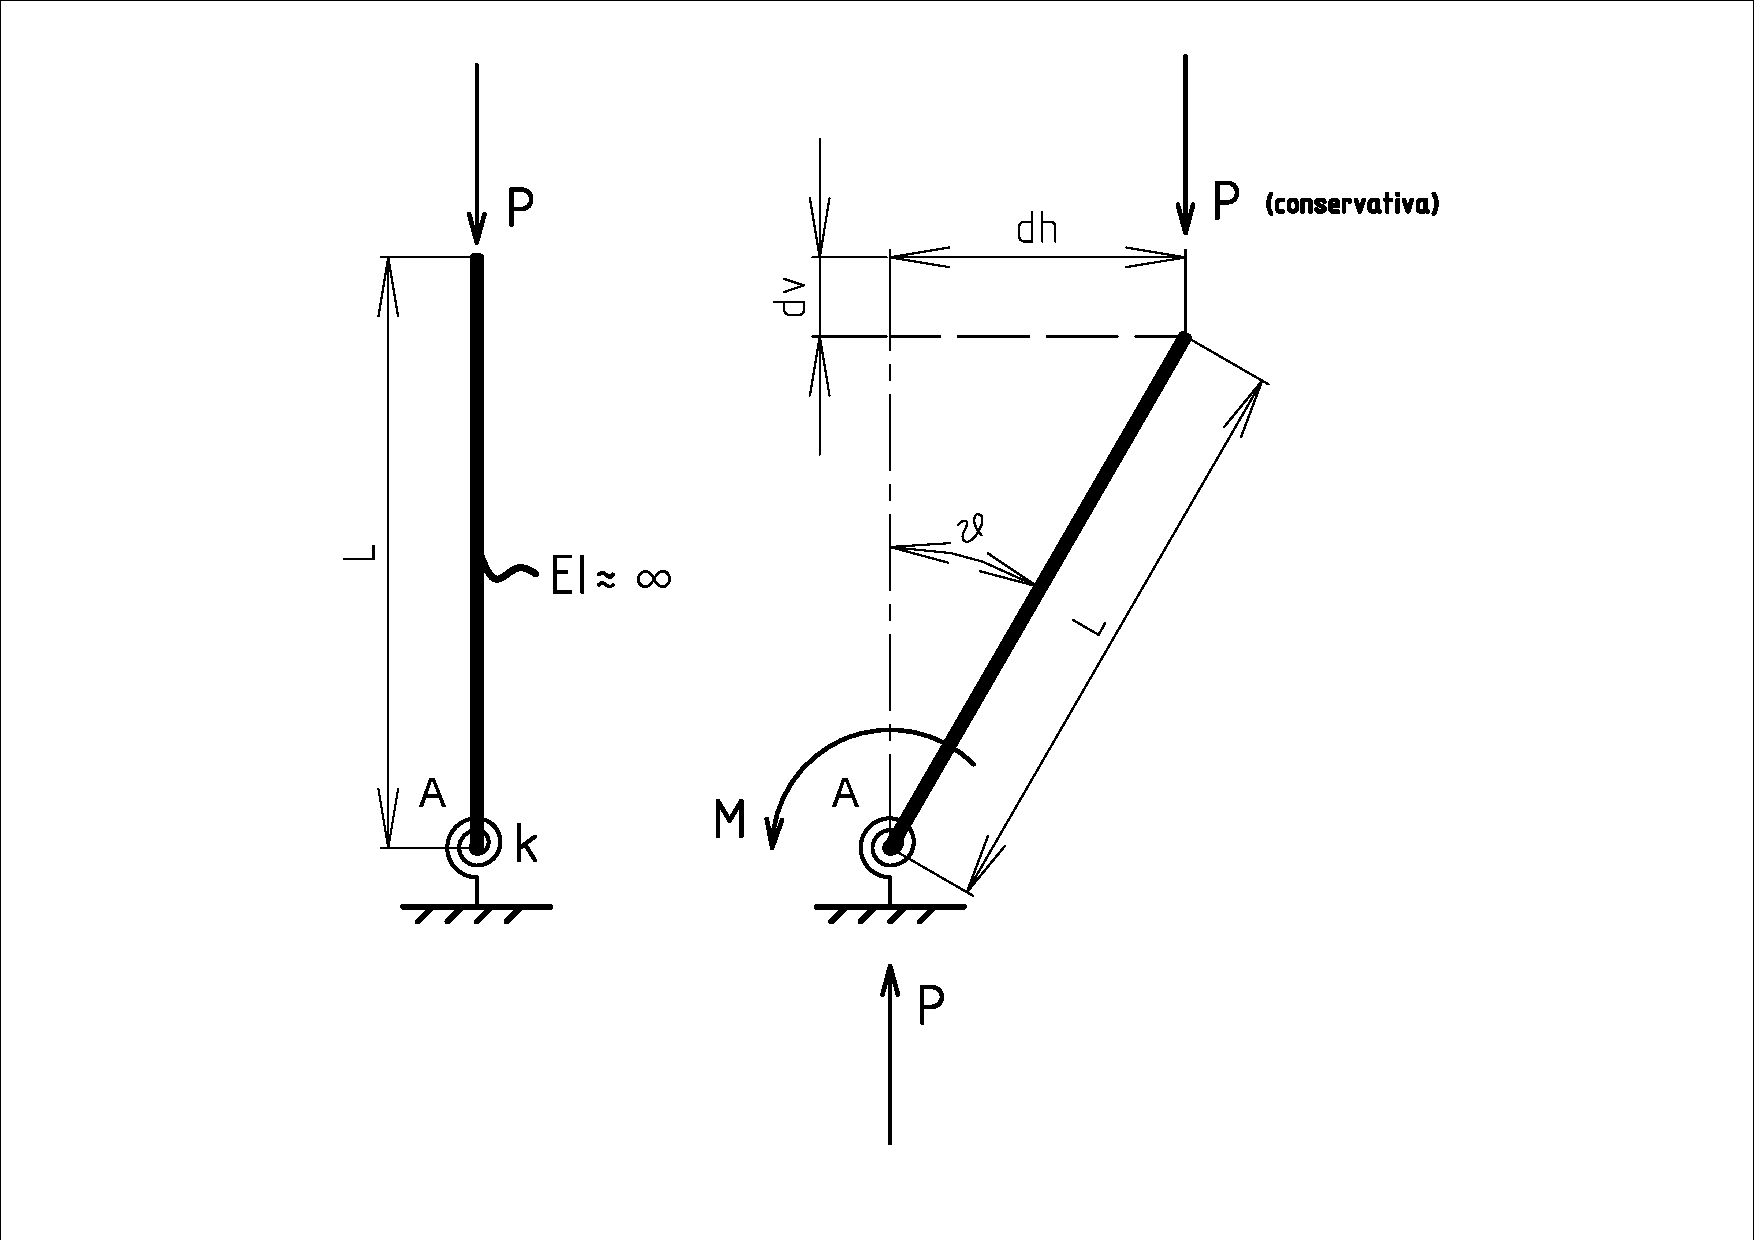
\includegraphics[
		trim=55mm 15mm 50mm 8mm,
		clip,
		width=0.73\textwidth
	]{figuras/TPs-1.pdf}
	\label{fig:TP1}
\end{figure}


% ================ Resolução TP-01 ================
\begin{textocaixa}
\hspace{10mm}
O sistema estrutural da barra rígida acoplada à uma mola de torção, de rigidez $K_\text{mola}$
na base, quando assumido possuir grandes deslocamentos, possui como solução geral para o
problema de determinação da carga $P$, aplicada verticalmente de forma conservativa na
extremidade livre da barra, a qual equilibra o sistema a expressão dada na
\autoref{eq:TP1-P_theta}.

\begin{equation}
	P = \frac{k_\text{mola}}{L}\frac{\theta}{\sin \theta}
	\label{eq:TP1-P_theta}
\end{equation}

Ainda, aplicando relações trigonométricas na geometria do sistema estrutural na condição de
equilíbrio, pode-se expressar o valor da carga em função dos deslocamentos vertical
($\delta_v$) e horizontal ($\delta_h$):

\begin{equation}
	\left\{\begin{array}{lcl}
		\delta_v &=& L\left(1 - \cos \theta\right) \\
		\delta_h &=& L\sin \theta \\
	\end{array}\right.
	\label{eq:TP1-deltavh}
\end{equation}

As fórmulas foram implementadas no MATLAB$^\text{\textregistered}$ para visualização gráfica
do comportamento não-linear geométrico (NLG) da estrutura, de acordo com os valores dados no
enunciado. Os gráficos $P\times\theta$, $P\times \delta_v$ e $P\times \delta_h$ são mostrados
na \autoref{fig:TP1-result}.

\begin{figure}[H]
	\centering
	\caption{TP1 $-$ Curvas do carregamento vertical $P$.}
	
\includegraphics[
		width=\textwidth
	]{figuras/no_image.png}
	\caption*{Fonte: Autor}
	\label{fig:TP1-result}
\end{figure}

As linhas de código que geraram estes gráficos estão disponíveis no \autoref{apendice:A}.

\end{textocaixa}
% ============================================== %

%%%%%%%%%%%%%%%%%%%%%%%%%%%%%%%%%%%%%%%%%%%%%%%%%%
%%%			  02 Trabalho Prático 02		   %%%
%%%%%%%%%%%%%%%%%%%%%%%%%%%%%%%%%%%%%%%%%%%%%%%%%%

% ============================================== %

\section{Trabalho Prático 02}


Uma barra rígida biapoiada possui apoio elástico de translação no topo. Pede-se traçar os
gráficos de força aplicada ($P$) \textit{versus} deslocamento horizontal
($\delta_\mathrm{H}$) e vertical ($\delta_\mathrm{V}$)  referentes ao ponto de aplicação
da força. Adotar:

$$
\left\{\begin{array}{lcl}
	k_\text{mola} &=& 1\:\:\text{kN/cm} \\
	L &=& 100\:\:\text{cm} \\
	\Delta\theta &=& \frac{\pi}{90}\:\:\text{rad} \\
\end{array}\right.
$$

\begin{figure}[H]
	\centering
	\caption{Sistema estrutural do Trabalho Prático 02.}
	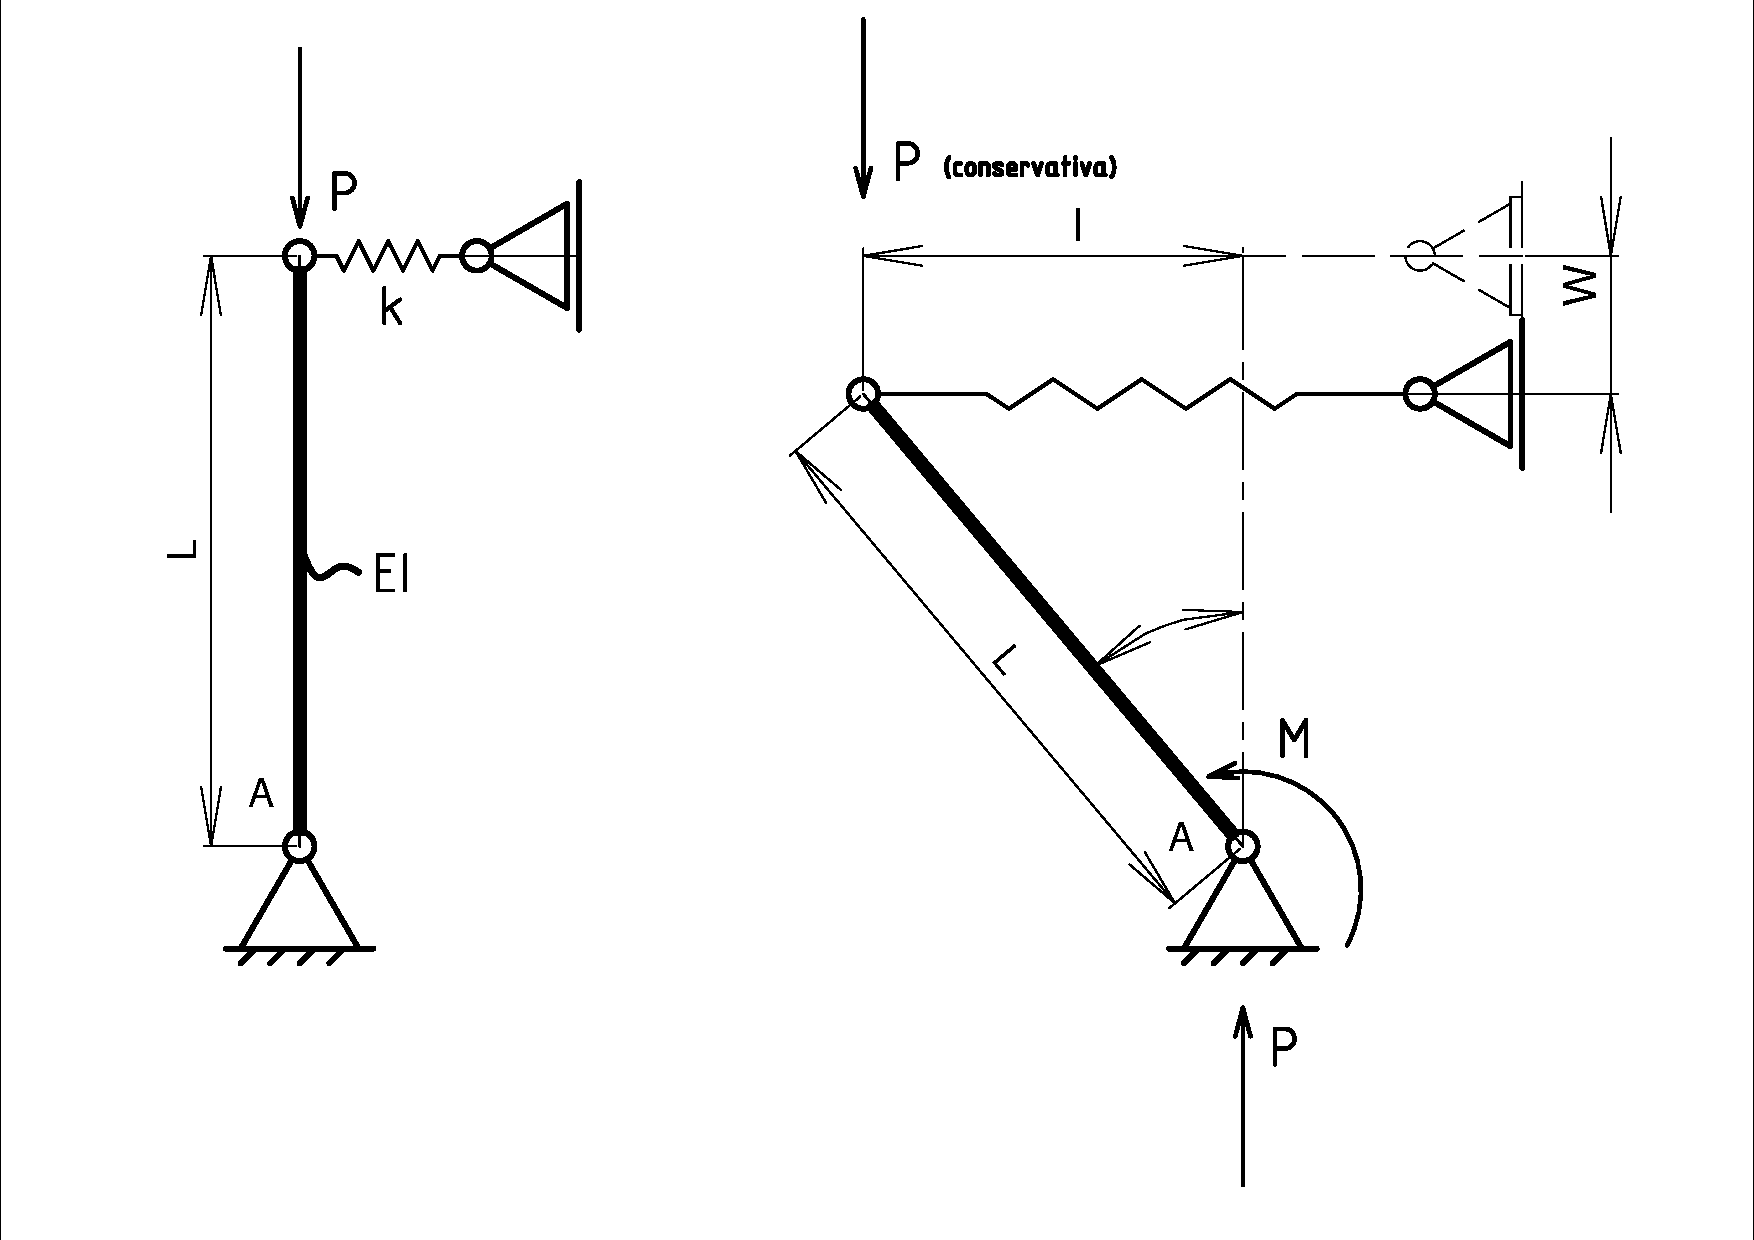
\includegraphics[
		trim=25mm 8mm 2mm 3mm,
		clip,
		width=\textwidth
	]{figuras/TPs-2.pdf}
	\label{fig:TP2}
\end{figure}


% ================ Resolução TP-02 ================
\begin{textocaixa}
\hspace{10mm}

Neste sistema estrutural, assume-se, novamente, \underline{relação constitutiva} linear da
mola:

\begin{equation}
	F_\text{mola} = k_\text{mola}\cdot \delta_h
	\label{eq:TP2-const}
\end{equation}

E como \underline{relações cinemáticas}, tem-se a associação entre as variações $\delta_h$
e $\delta_v$ com o ângulo de giro $\theta$ da barra por meio da \autoref{eq:TP2-cinem}.

\begin{equation}
	\left\{\begin{array}{lcl}
		\delta_h &=& L\sin \theta \\
		\delta_v &=& L\left(1 - \cos\theta\right) \\
	\end{array}\right.
	\label{eq:TP2-cinem}
\end{equation}

Assim, o equilíbrio de momentos em relação ao apoio fixo A resultam na carga $P$ em função do
ângulo $\theta$ dado na \autoref{eq:TP2-P_theta}, assumindo grandes deslocamentos.

\begin{equation}
	P = k_\text{mola}\,L\cdot \cos\theta
	\label{eq:TP2-P_theta}
\end{equation}

Graficamente, essa relação não-linear é expressa pelas curvas $P\times \delta_v$ e
$P\times \delta_h$ mostradas na \autoref{fig:TP2-result}, geradas pelo código dado em
\autoref{subapendice:TP02}.

\begin{figure}[H]
	\centering
	\caption{TP02 $-$ Curvas do carregamento vertical $P$.}
	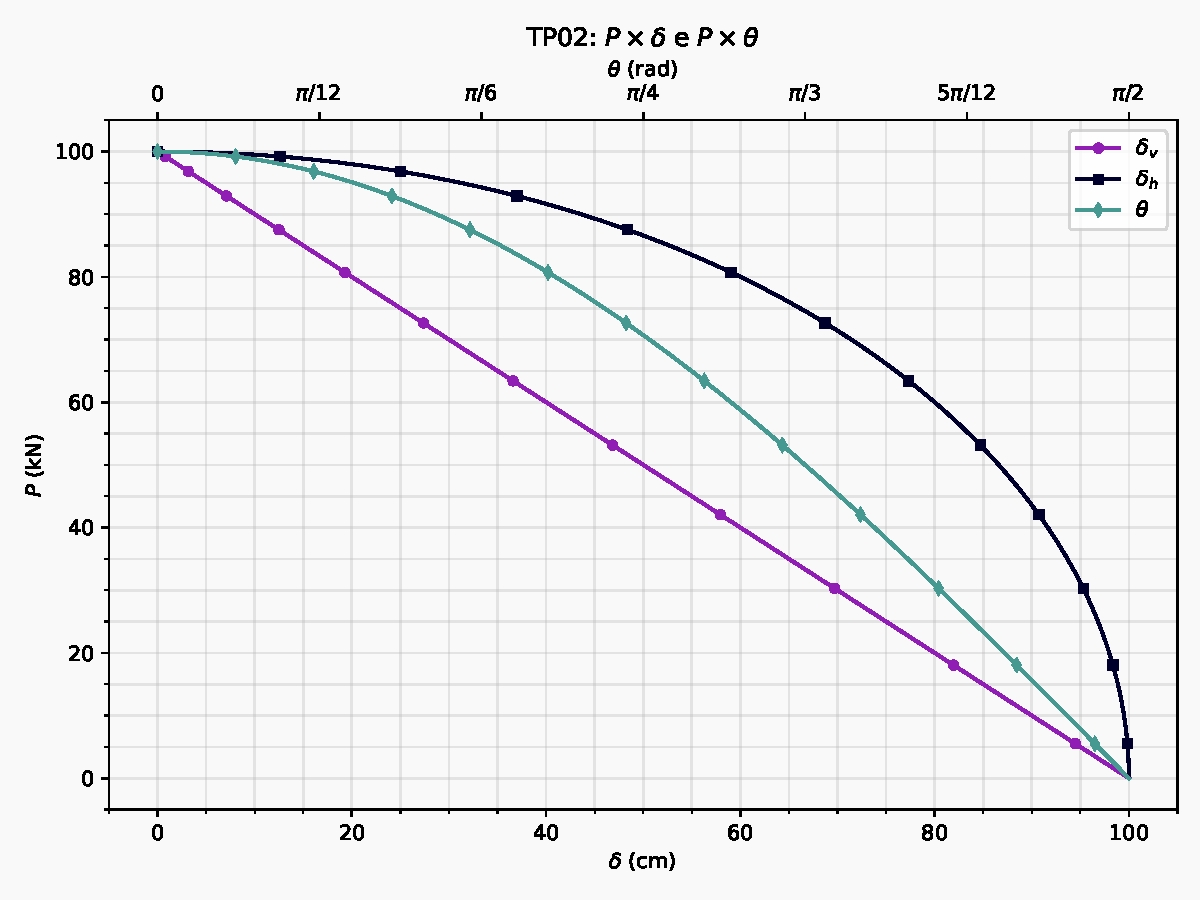
\includegraphics[
		width=\textwidth
	]{figuras/resultados/TP02-result.pdf}
	\label{fig:TP2-result}
\end{figure}

Nesse sistema estrutural, a carga crítica se relaciona com as constantes do problema da
seguinte forma:

\begin{equation}
	P_{cr} = \lim_{\theta\:\longrightarrow\:0} k_\text{mola}\,L\cdot \cos\theta
	\Longrightarrow \boxed{P_{cr} = k_\text{mola}\,L}
	\label{eq:TP2-P_cr}
\end{equation}



\end{textocaixa}
% ============================================== %

%%%%%%%%%%%%%%%%%%%%%%%%%%%%%%%%%%%%%%%%%%%%%%%%%%
%%%			  03 Trabalho Prático 03		   %%%
%%%%%%%%%%%%%%%%%%%%%%%%%%%%%%%%%%%%%%%%%%%%%%%%%%

% ============================================== %

\section*{Trabalho Prático 03}


Fazer os gráficos $P\times\delta_\mathrm{V}$, $P\times\delta_\mathrm{H}$, $P\times\theta$
para $\theta \in \left[0, \frac{\pi}{2}\right]$. Adotar:

$$
\left\{\begin{array}{lcl}
	k &=& 1000\text{ kN}\cdot\text{cm/rad} \\
	L &=& 100\:\:\text{cm} \\
	\Delta\theta &=& \frac{\pi}{36}\:\:\text{rad} \\
\end{array}\right.
$$

\begin{figure}[H]
	\centering
	\caption{Sistema estrutural do Trabalho Prático 3.}
	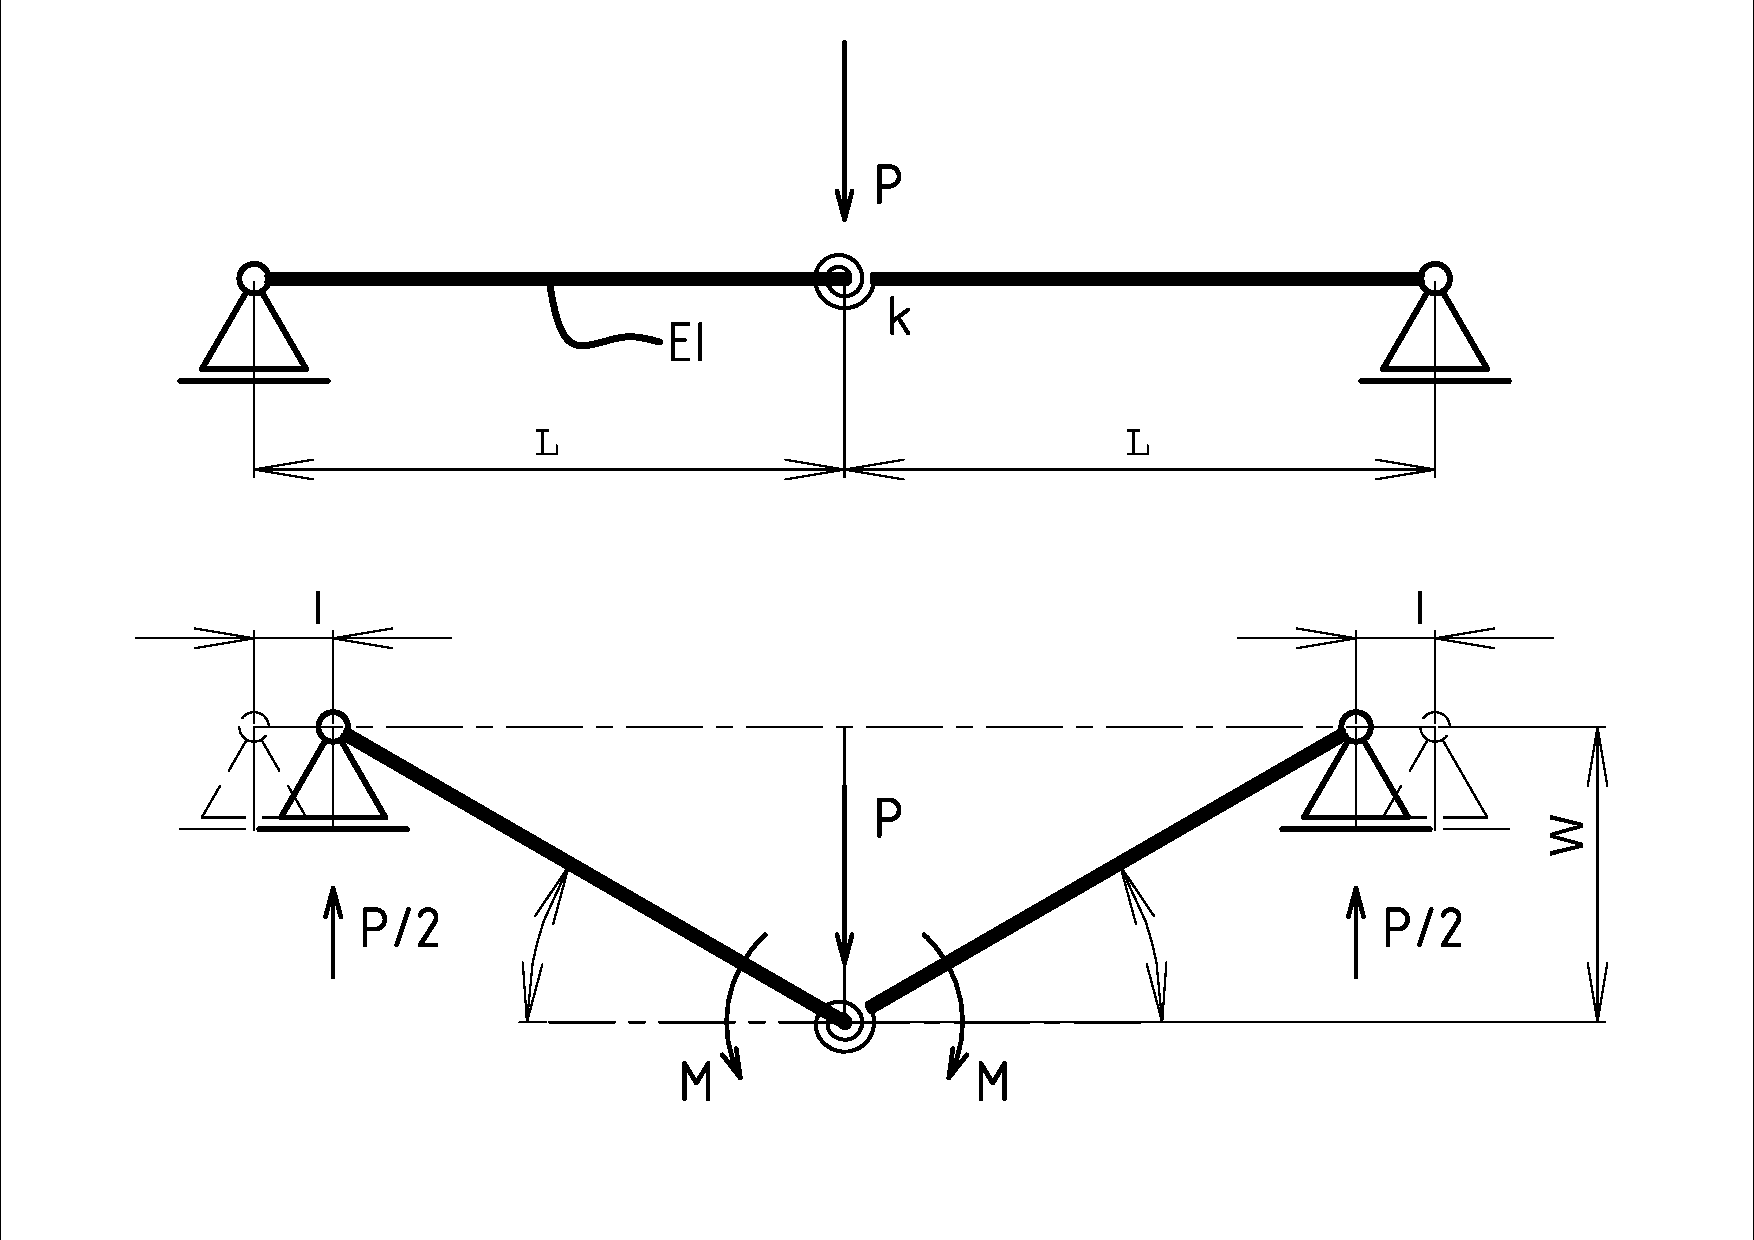
\includegraphics[
		trim=20mm 20mm 20mm 5mm,
		clip,
		width=\textwidth
	]{figuras/TPs-3.pdf}
\end{figure}


% ================ Resolução TP-03 ================
\begin{textocaixa}
\hspace{10mm}




\end{textocaixa}
% ============================================== %

%%%%%%%%%%%%%%%%%%%%%%%%%%%%%%%%%%%%%%%%%%%%%%%%%%
%%%			  04 Trabalho Prático 04		   %%%
%%%%%%%%%%%%%%%%%%%%%%%%%%%%%%%%%%%%%%%%%%%%%%%%%%

% ============================================== %

\section{Trabalho Prático 04}


Para a viga engastada com momento constante aplicado na extremidade livre pede-se:

\begin{itemize}
	\item[a)] Traçar os gráficos $M\times \theta$, $M\times u$, $M\times v$ para
	$\pi \in \left[0, 2\pi\right]$ rad no ponto $x=L$
	\item[b)] Detalhar a solução da viga deformada para $\theta = \pi$ e
	$\theta = 2\pi$, considerando-se 11 pontos igualmente espaçados (10 elementos)
	ao longo do comprimento da viga.
\end{itemize}

Adotar:
$$
\left\{\begin{array}{lcl}
	EI &=& 4\times 10^4\text{ N/cm} \\
	L &=& 500\text{ cm} \\
	\Delta\theta &=& \frac{\pi}{36}\:\:\text{rad} \\
\end{array}\right.
$$

\begin{figure}[H]
	\centering
	\caption{Sistema estrutural do Trabalho Prático 04.}
	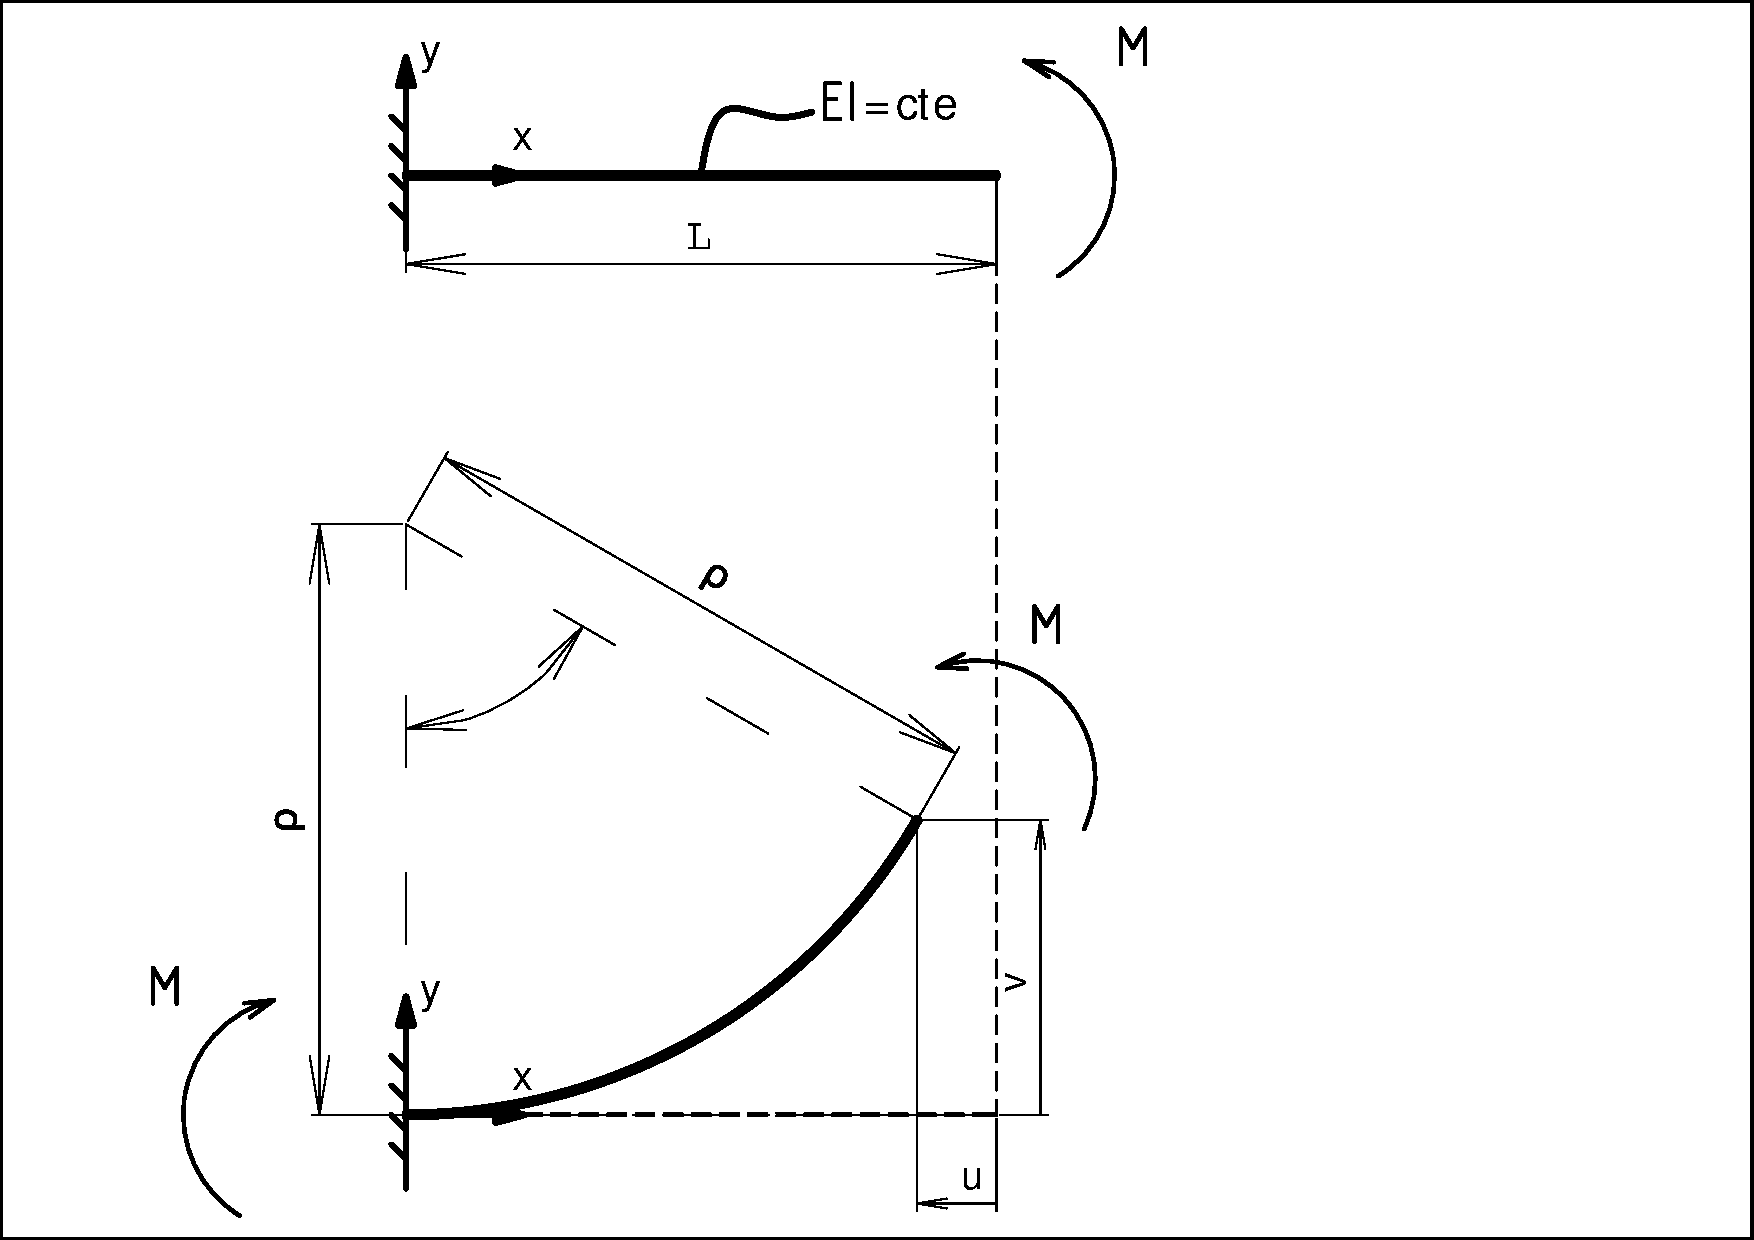
\includegraphics[
		trim=25mm 3mm 100mm 4mm,
		clip,
		width=0.75\textwidth
	]{figuras/TPs-4.pdf}
\end{figure}


% ================ Resolução TP-04 ================
\begin{textocaixa}
\hspace{10mm}




\end{textocaixa}
% ============================================== %

%%%%%%%%%%%%%%%%%%%%%%%%%%%%%%%%%%%%%%%%%%%%%%%%%%
%%%			  05 Trabalho Prático 05		   %%%
%%%%%%%%%%%%%%%%%%%%%%%%%%%%%%%%%%%%%%%%%%%%%%%%%%

% ============================================== %

\section{Trabalho Prático 05}

Fazer os gráficos $F\times \delta_v$ (deslocamento vertical) e $N\times \delta_v$ para
$y \in \left[0,40; 0,20\right]$ m. Adotar:

$$
\left\{\begin{array}{lcl}
	\Delta y &=& -0,01\text{ m} \\
	EA_0 &=& 133,865\text{ kN} \\
	L &=& 4,0\text{ m} \\
	H &=& 0,20\text{ m} \\
\end{array}\right.
$$

\begin{figure}[H]
	\centering
	\caption{Sistema estrutural do Trabalho Prático 05.}
	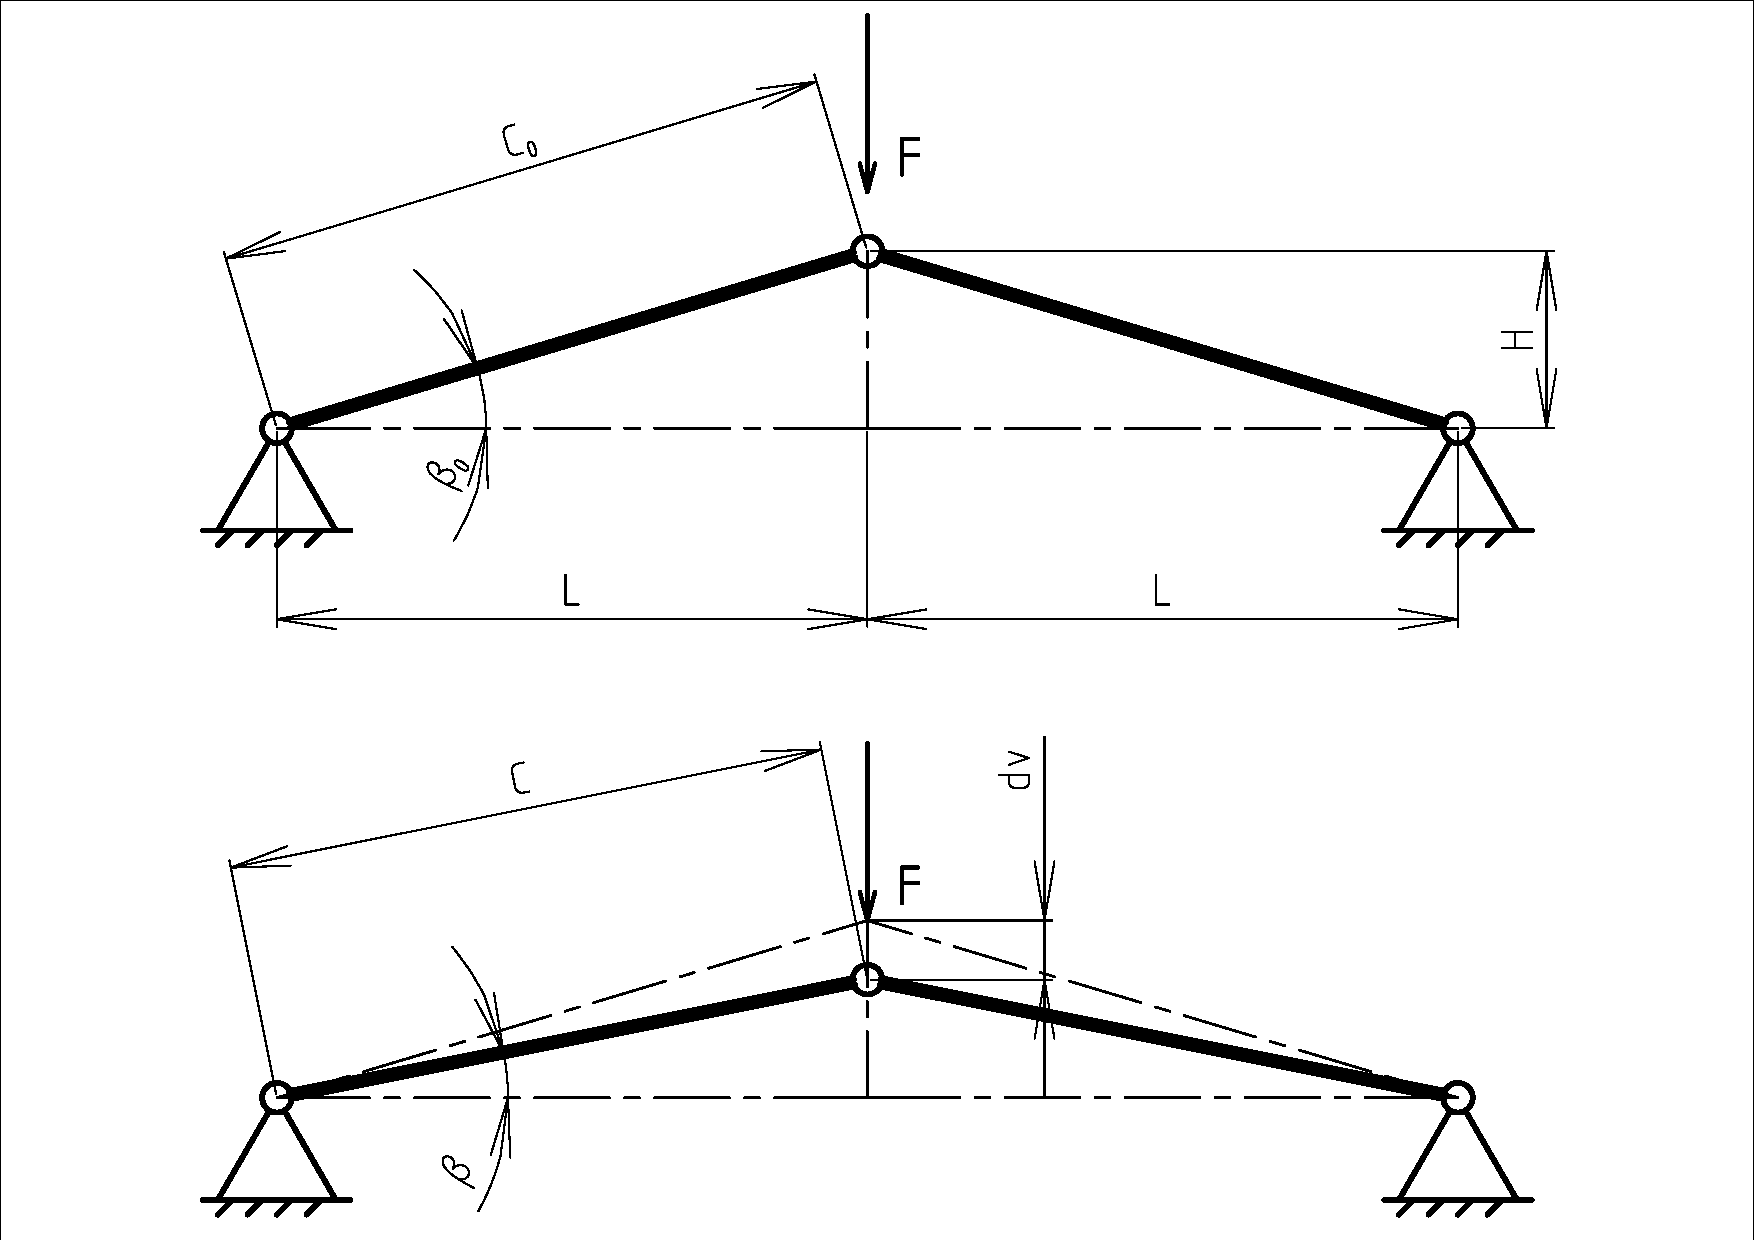
\includegraphics[
		trim=30mm 4mm 30mm 2mm,
		clip,
		width=0.75\textwidth
	]{figuras/TPs-5.pdf}
\end{figure}


% ================ Resolução TP-05 ================
\begin{textocaixa}
\hspace{10mm}




\end{textocaixa}
% ============================================== %

%%%%%%%%%%%%%%%%%%%%%%%%%%%%%%%%%%%%%%%%%%%%%%%%%%
%%%			  06 Trabalho Prático 06		   %%%
%%%%%%%%%%%%%%%%%%%%%%%%%%%%%%%%%%%%%%%%%%%%%%%%%%

% ============================================== %

\section{Trabalho Prático 06}

Fazer gráficos de (1.) estiramento ($\lambda$) \textit{versus} medidas de deformação clássicas
e (2.) estiramento \textit{versus} conjugados de tensão normalizados $\displaystyle\left(
\frac{\sigma^*}{\sigma_B}\right)$ para $\lambda \in \left]0; 2\right]$.


% ================ Resolução TP-06 ================
\begin{textocaixa}
\hspace{10mm}




\end{textocaixa}
% ============================================== %

%%%%%%%%%%%%%%%%%%%%%%%%%%%%%%%%%%%%%%%%%%%%%%%%%%
%%%			  07 Trabalho Prático 07		   %%%
%%%%%%%%%%%%%%%%%%%%%%%%%%%%%%%%%%%%%%%%%%%%%%%%%%

% ============================================== %

\section{Trabalho Prático 07}

\begin{enumerate}
    \item Calcular as energias de deformação específicas para as medidas de deformação
    Logarítmica e de Green.
    \item Encontrar os valores das constantes para leis do tipo: $\sigma^* = E\cdot
    \varepsilon^*$ (leis Hookeanas).
\end{enumerate}

% ================ Resolução TP-07 ================
\begin{textocaixa}
\hspace{10mm}

A energia de deformação específica $u^*$ se relaciona com o estiramento $\lambda$ a partir
da \autoref{eq:TP7-energia}.

\begin{equation}
    u^* = \int_{\varepsilon^*}\sigma^*\,\mathrm{d}\varepsilon^*
        = \int_\lambda \left(\sigma^*\:\frac{\partial \varepsilon^*}
                                            {\partial \lambda}\right)\,\mathrm{d}\lambda
    \label{eq:TP7-energia}
\end{equation}

Em consequência, considerando lei constitutiva Hookeana para os pares de tensão-deformação,
a expressão para o cálculo da energia de deformação específica se transforma em:

\begin{equation}
    u^* = E\:\int_\lambda \left(\varepsilon^*\:
                                \frac{\partial \varepsilon^*}
                                     {\partial \lambda}\right) \mathrm{d}\lambda
    \label{eq:TP7-energia_estiramento}
\end{equation}

Ou, então, numa relação direta com a deformação $\varepsilon^*$, dada na
\autoref{eq:TP7-energia_deform}, que será utilizada nesta resolução.

\begin{equation}
    u^* = E\:\int_{\varepsilon^*} \left(E\cdot\varepsilon^*\right)
                                      \,\varepsilon^* \mathrm{d}\varepsilon^*
    \longrightarrow \boxed{u^* = \frac{E}{2}\left[\varepsilon^*\left(\lambda\right)\right]^2}
    \label{eq:TP7-energia_deform}
\end{equation}

\begin{enumerate}
    \item \underline{Energia de deformação específica}

A medida de deformação Logarítmica $\varepsilon^* = \varepsilon_L$ é expressa por:

\begin{equation}
    \varepsilon_L = \ln \lambda
    \label{eq:TP7-eL}
\end{equation}

Implicando que a energia de deformação para a medida de deformação Logarítmica é dada por:

\begin{equation}
    \boxed{u_L = \frac{E}{2}\left(\ln\lambda\right)^2}
    \label{eq:TP7-uL_general}
\end{equation}

Já a medida de deformação de Green se expressa na \autoref{eq:TP7-eG}, permitindo desenvolver
a expressão para a energia de deformação específica para esta medida de deformação ($u_G$)
na \autoref{eq:TP7-uG}.

\begin{equation}
    \varepsilon_G = \frac{1}{2}\left(\lambda^2 - 1\right)
    \label{eq:TP7-eG}
\end{equation}

\begin{equation}
    \Longrightarrow u_G = \frac{E}{2}\left[\frac{1}{2}\left(\lambda^2 - 1\right)\right]^2
    \longrightarrow
    \boxed{u_G = \frac{E\,\lambda^2}{8}\left(\lambda^2 - 2\right) + \frac{E}{8}}
    \label{eq:TP7-uG}
\end{equation}

\item \underline{Constantes para leis do tipo Hookeanas}

Os conjugados de tensão de cada medida da deformação clássica se relacionam com a tensão de
Biot $\sigma_B$, dada na \autoref{eq:TP7-sigmaB}, a partir de expressões envolvendo o
estiramento.

\begin{equation}
    \sigma_B = E\left(\lambda - 1\right)
    \label{eq:TP7-sigmaB}
\end{equation}

Para as medidas de deformação Logarítmica e de Green, essas relações são mostradas na
\autoref{eq:TP7-sigmaLGB}.

\begin{bigEquation}
    \left\{\begin{array}{lclcl}
        \sigma_L &=& \lambda\,\sigma_B &=& 
                     E\cdot \left(\lambda^2 - \lambda\right) \\ [10pt]
        \sigma_G &=& \frac{1}{\lambda}\,\sigma_B &=& 
                     E\cdot \left(1 -\frac{1}{\lambda}\right) \\
    \end{array}\right.
    \label{eq:TP7-sigmaLGB}
\end{bigEquation}

Além disso, considerando a constante de proporcionalidade $E_L$ para a medida de deformação
Logarítmica e $E_G$ para a medida de deformação de Green, as leis constitutivas equivalente
são expressas como:

\begin{bigEquation}
    \left\{\begin{array}{lclcl}
        \sigma_L &=& E_L\cdot\varepsilon_L &=& 
                     E_L\cdot \ln\lambda \\ [10pt]
        \sigma_G &=& E_G\cdot\varepsilon_G &=& 
                     E_G\cdot \frac{1}{2}\left(\lambda^2 - 1\right) \\
    \end{array}\right.
    \label{eq:TP7-sigmaLG_const}
\end{bigEquation}

Portanto, comparando-se a \autoref{eq:TP7-sigmaLG_const} com a \autoref{eq:TP7-sigmaLGB},
encontram-se relações entre as constantes de proporcionalidade e o módulo de Young $E$
referente à medida de deformação de Biot -- a qual está ligada a ensaios de caracterização
que medem a deformação com base nas dimensões iniciais. Para a medida de deformação
Logarítmica, tem-se, pois, que:

\begin{equation}
    \frac{E_L}{E} = \frac{\lambda^2 - \lambda}{\ln\lambda}
    \label{eq:TP7-EL_E}
\end{equation}

Enquanto, para a medida de deformação de Green, a razão entre $E_G$ e $E$ se torna:

\begin{equation}
    \frac{E_G}{E} = \frac{2}{\lambda^2 + \lambda}
    \label{eq:TP7-EG_E}
\end{equation}

Retomando esse resultado na \autoref{eq:TP7-sigmaLGB}, as leis constitutivas do tipo
Hookeanas para as medidas de deformação Logarítmica e de Green são formuladas na
\autoref{eq:TP7-sigmaL_hook} e \autoref{eq:TP7-sigmaG_hook}, respectivamente.

\begin{equation}
    \boxed{\sigma_L = \frac{\lambda^2 - \lambda}{\ln\lambda}\,E\cdot \varepsilon_L}
    \label{eq:TP7-sigmaL_hook}
\end{equation}

\begin{equation}
    \boxed{\sigma_G = \frac{2E}{\lambda^2 + \lambda}\cdot \varepsilon_G}
    \label{eq:TP7-sigmaG_hook}
\end{equation}

\end{enumerate}



\end{textocaixa}
% ============================================== %

%%%%%%%%%%%%%%%%%%%%%%%%%%%%%%%%%%%%%%%%%%%%%%%%%%
%%%			  08 Trabalho Prático 08		   %%%
%%%%%%%%%%%%%%%%%%%%%%%%%%%%%%%%%%%%%%%%%%%%%%%%%%

% ============================================== %

\section{Trabalho Prático 08}

Para a treliça espacial simétrica de 3 barras, pede-se fazer gráficos $P\times\delta_v$ (
deslocamento vertical) e $P\times N$ (força axial nas barras) considerando-se $y \in [-4; 2]$
m usando as cinco leis constitutivas que relacionam linearmente as medidas de deformação
clássicas e seus respectivos pares conjugados de tensão. Adotar:

$$
\left\{\begin{array}{lcl}
	EA_0 &=& 133,865\text{ kN} \\
	H &=& 200\text{ cm} \\
	L &=& 500\text{ cm} \\
	\Delta y &=& -0,02\text{ m} \\
\end{array}\right.
$$

\begin{figure}[H]
	\centering
	\caption{Sistema estrutural do Trabalho Prático 08 -- Vista superior}
	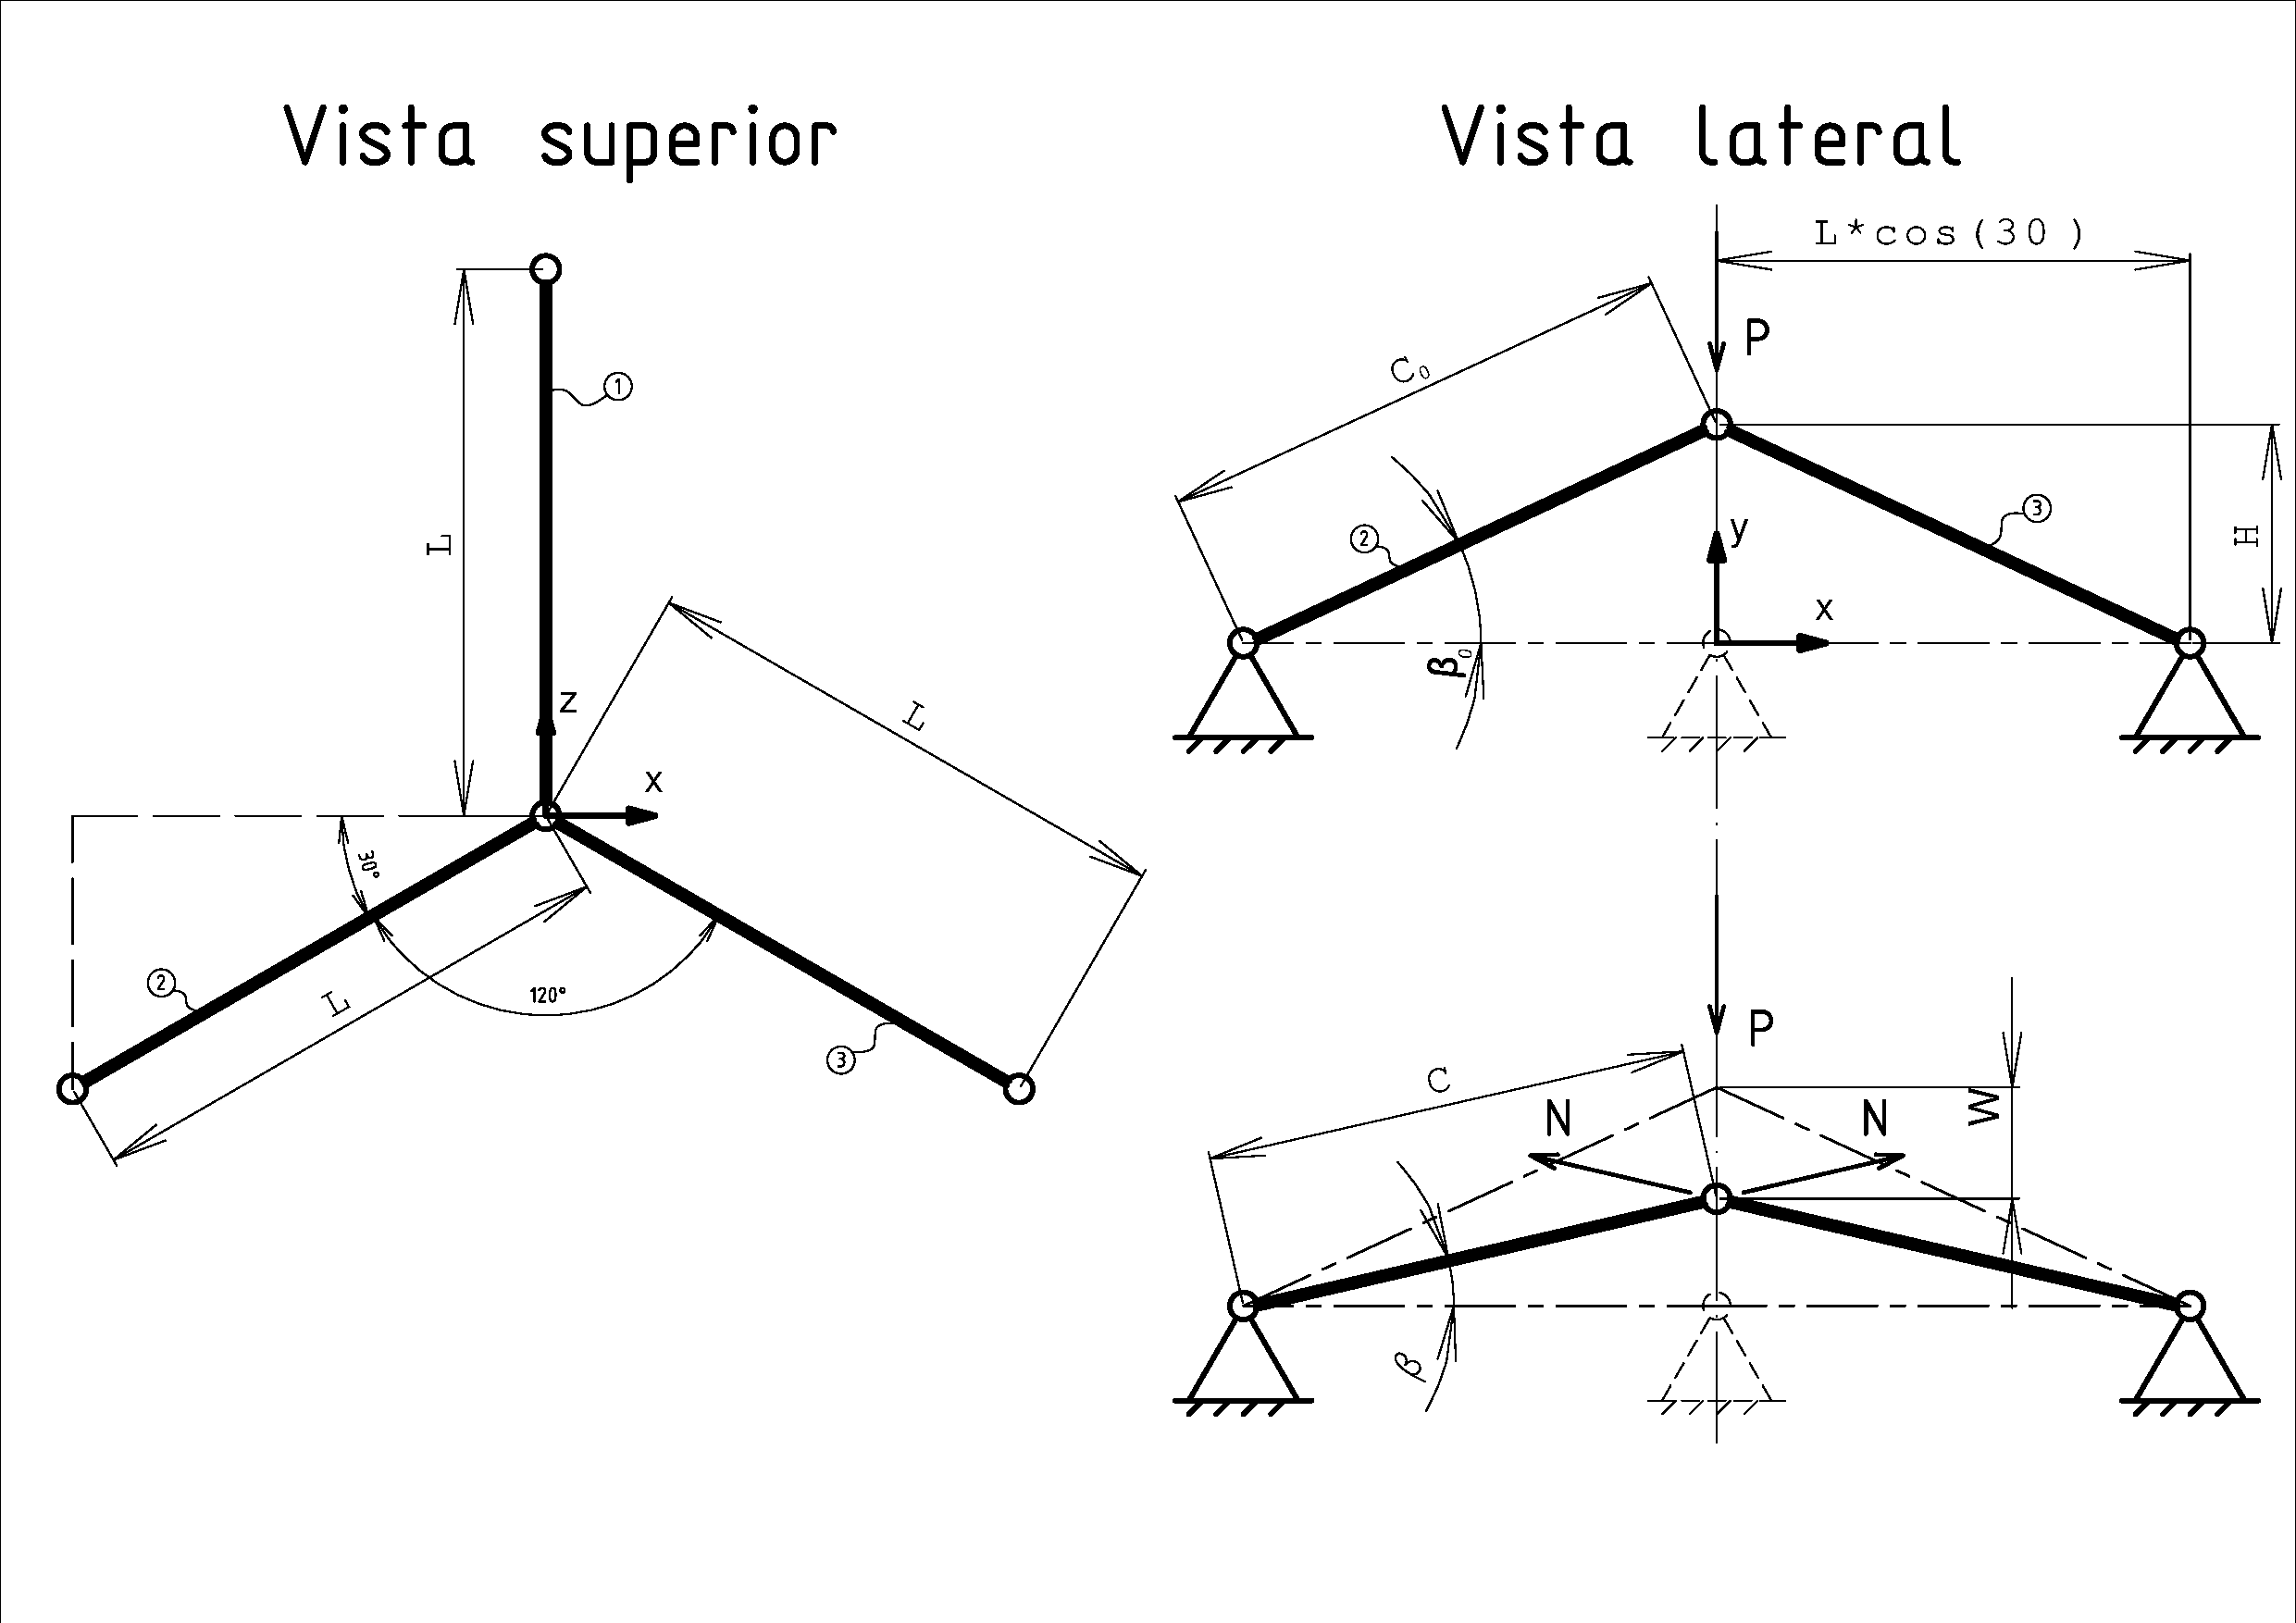
\includegraphics[
		trim=8mm 75mm 210mm 40mm,
		clip,
		width=0.75\textwidth
	]{figuras/TPs-8.pdf}
\end{figure}

\begin{figure}[H]
	\centering
	\caption{Sistema estrutural do Trabalho Prático 08 -- Vista lateral}
	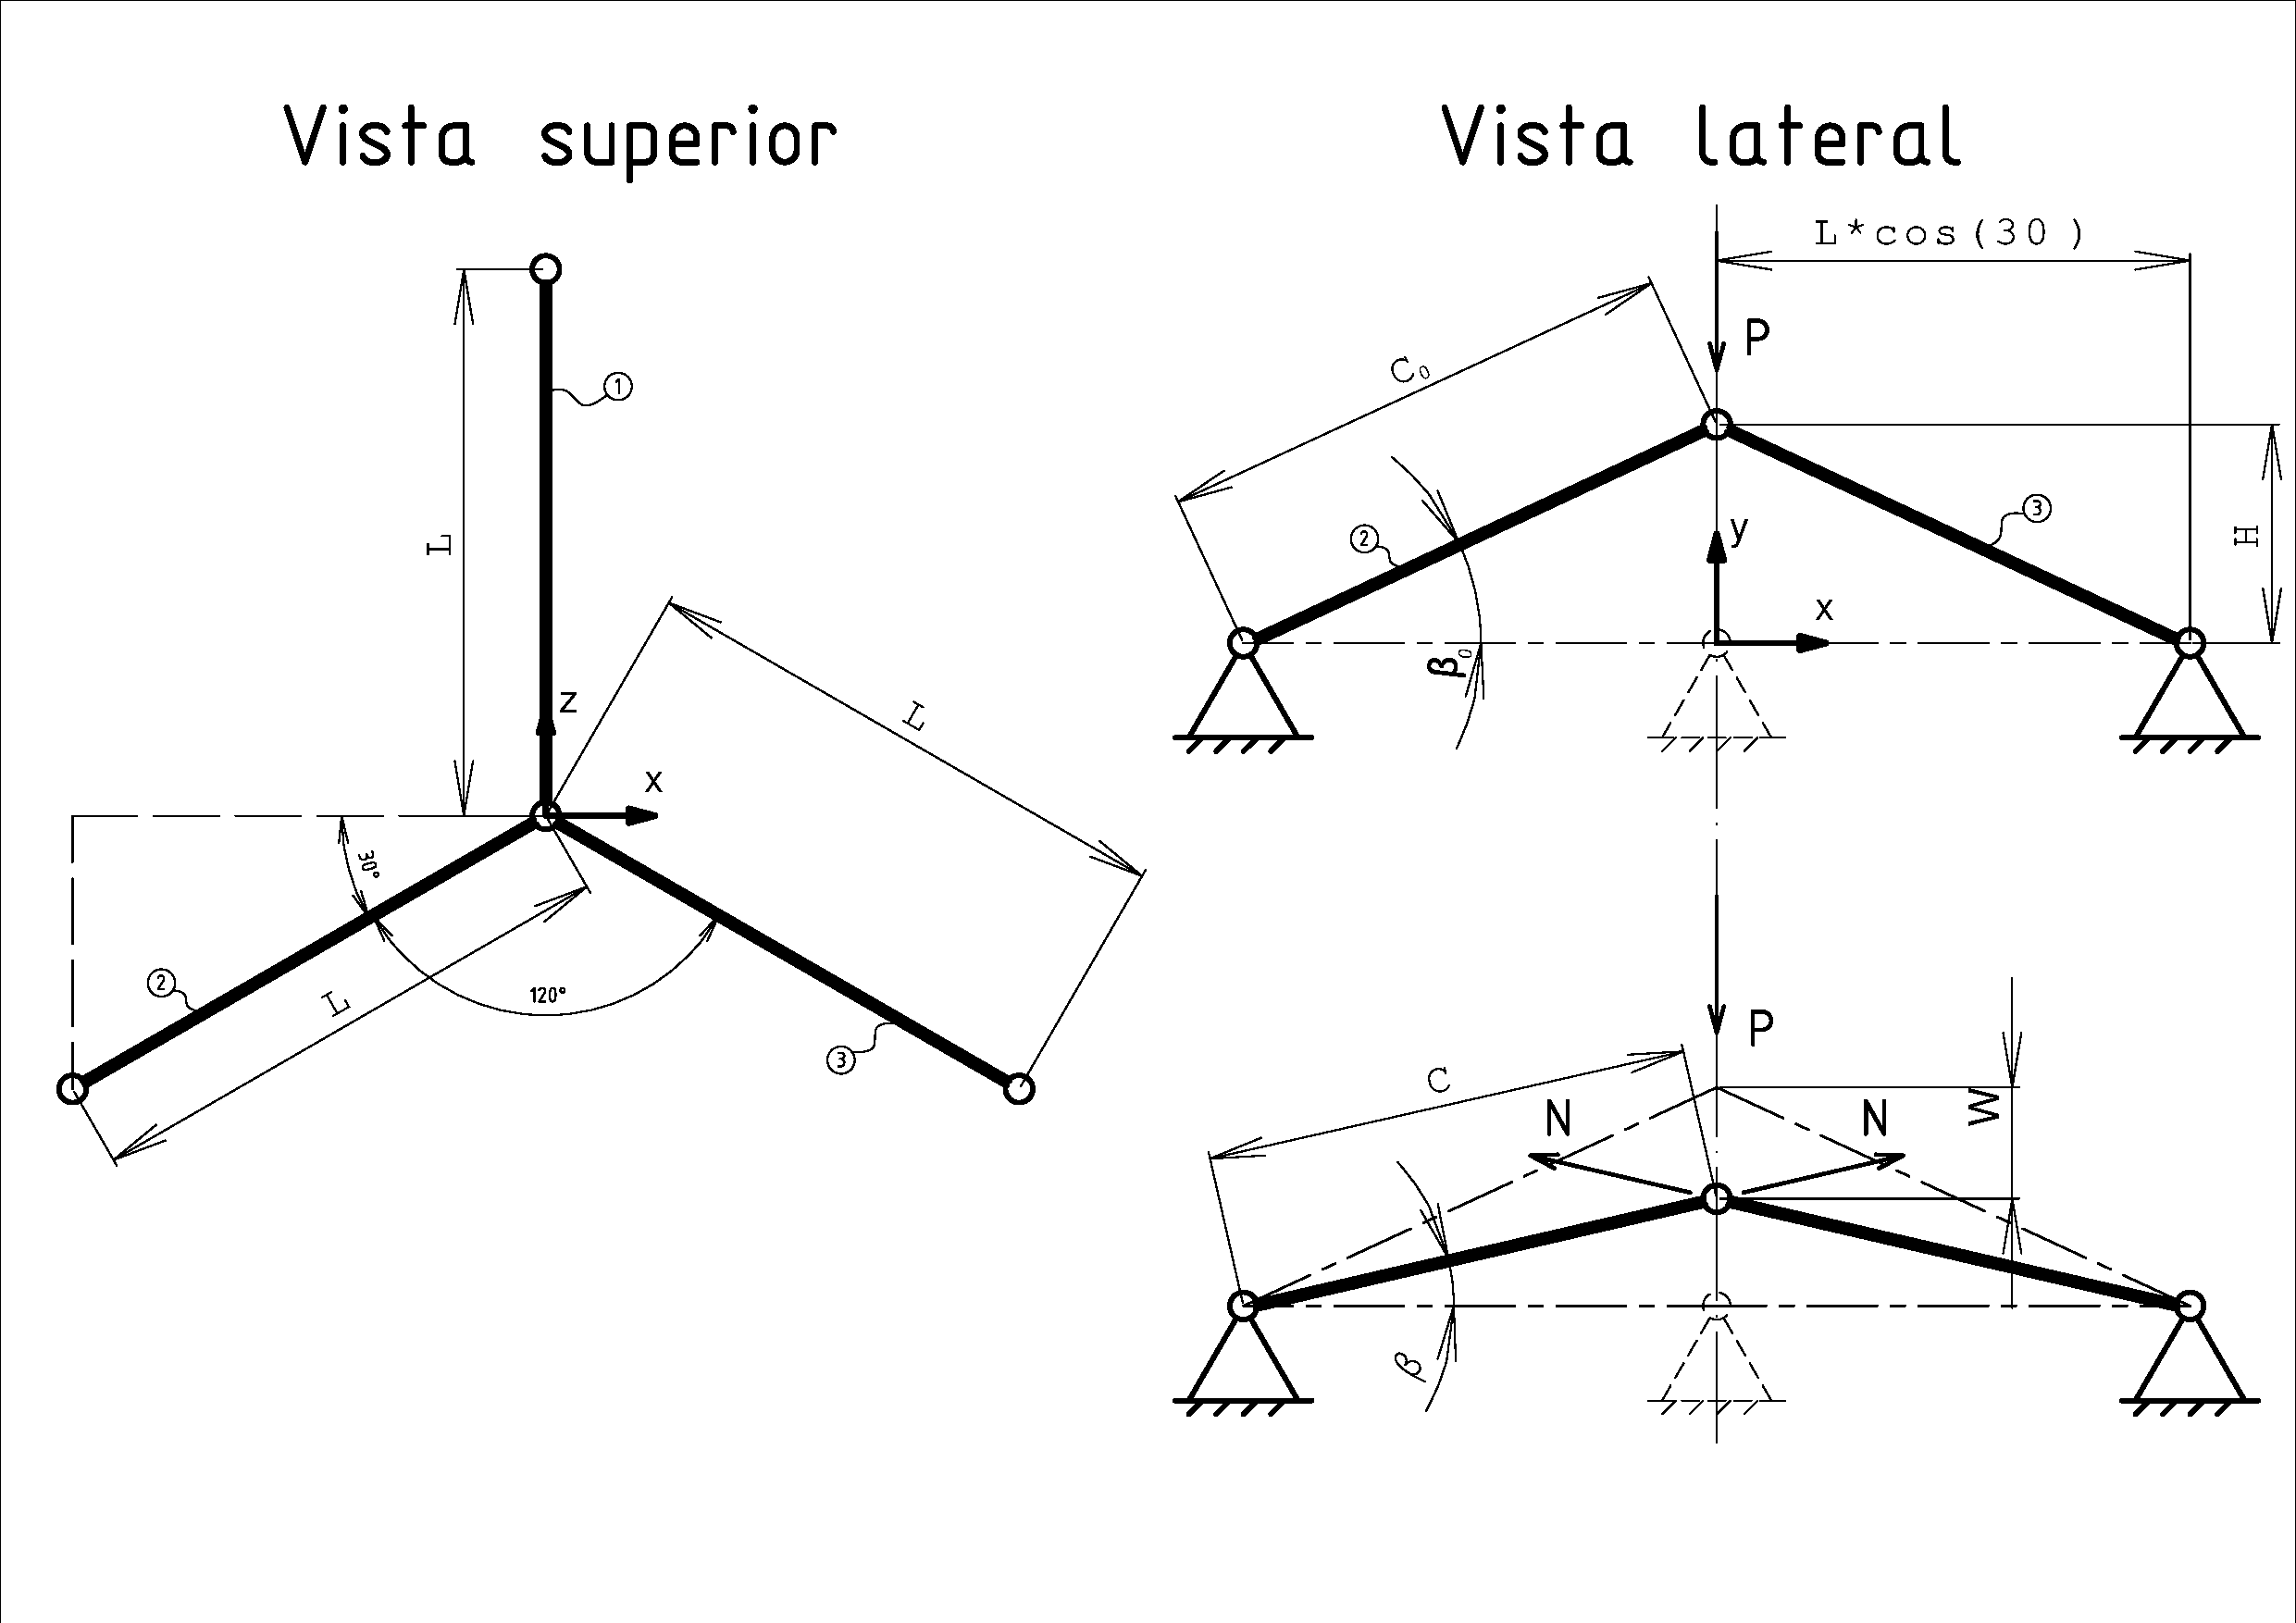
\includegraphics[
		trim=210mm 35mm 1.5mm 35mm,
		clip,
		width=0.85\textwidth
	]{figuras/TPs-8.pdf}
\end{figure}


% ================ Resolução TP-08 ================
\begin{textocaixa}
\hspace{10mm}

A treliça espacial do problema possui simetria radial, de modo que a força normal
$\vv{N} = \left(N_x\,\hat{i} + N_y\,\hat{j} + N_z\,\hat{k}\right)$, atuante na direção axial
de cada barra, possui o mesmo módulo para todas as barras. No \underline{equilíbrio}, a
resultante nas direções $x$ e $z$ das forças normais se cancelam, de modo que a equação de
equilíbrio se torna:

\begin{equation}
	3N_y - P = 0
	\label{eq:TP8-equi_init}
\end{equation}

Denotando por $\vv{v_1}$ o vetor direção da barra $\circled{1}$ na configuração deformada,
$\alpha$ o ângulo entre o vetor normal $\vv{N}$ e a vertical, e $N = ||\vv{N}||$,
tem-se que:

\begin{equation}
	\boxed{N_y = N\cos\alpha}
	\label{eq:TP8-Ny}
\end{equation}

\begin{equation}
	\cos\alpha = \frac{\left<\vv{v_1}, y\,\hat{j}\right>}
					  {||\vv{v_1}||\cdot
					   ||y\,\hat{j}||}
	= \frac{\left(0, y, L\right)\cdot\left(0, y, 0\right)}
		   {\sqrt{y^2 + L^2}\cdot y}
	\longrightarrow \boxed{\cos\alpha = \frac{y}{\sqrt{y^2 + L^2}}}
	\label{eq:TP8-cos_alpha}
\end{equation}

Por simetria, o ângulo $\alpha$ será igual para todas as barras. Assim, a equação final do
equilíbrio é dada por

\begin{equation}
	\boxed{N = -\frac{P}{3\cos\alpha}}
	\label{eq:TP8-equi}
\end{equation}

Além disso, as medidas de deformação clássicas (família Seth-Hill) se baseiam no estiramento
$\lambda$ da barra, no caso 1D, o qual é calculado como a razão entre o comprimento $c$ da
barra na configuração deformada e o comprimento $c_0$ da barra na configuração inicial:

\begin{equation}
	\lambda = \frac{c}{c_0}
	\label{eq:TP8-estiramento_init}
\end{equation}

Dimensões essas que se relacionam com os ângulos $\beta$ e $\beta_0$ baseando-se na
\underline{compatibilidade cinemática} do problema, dada na \autoref{eq:TP8-cinem}.

\begin{bigEquation}
	\left\{\begin{array}{lclcl}
		\tan\beta_0 &=& \frac{H}{L}    & & \\ [10pt]
		\tan\beta   &=& \frac{y}{L}    & & \\ [10pt]
		c_0			&=& L\,\sec\beta_0 &=& \sqrt{L^2 - H^2} \\ [10pt]
		c			&=& L\,\sec\beta   &=& \sqrt{L^2 - y^2}\\ [10pt]
	\end{array}\right.
	\label{eq:TP8-cinem}
\end{bigEquation}

Dessa forma, o estiramento se relaciona com os ângulos $\beta$ e $\beta_0$ de forma
não-linear, como mostrado na \autoref{eq:TP8-estiramento}.

\begin{equation}
	\lambda = \frac{c}{c_0} = \frac{L\,\sec\beta}{L\,\sec\beta_0}
	\longrightarrow \boxed{\lambda = \frac{\cos\beta_0}{\cos\beta}}
	\label{eq:TP8-estiramento}
\end{equation}

Ou, em termos das dimensões $L$, $H$ e $y$:

\begin{equation}
	\boxed{\lambda = \sqrt{\frac{\displaystyle 1 - \left(\frac{y}{L}\right)^2}
								{\displaystyle 1 - \left(\frac{H}{L}\right)^2}}}
	\label{eq:TP8-estiramento_alt}
\end{equation}

Enquanto o conjugado de tensão de cada medida de deformação se relaciona com a tensão de
Biot $\sigma_B$, a qual vale:

\begin{equation}
	\boxed{\sigma_B = \frac{N}{A_0}}
	\label{eq:TP8-sigmaB}
\end{equation}

Abaixo, serão construídas relações entre a carga $P$ e a coordenada $y$ do nó 4 (nó central)
para cada uma das cinco \underline{relações constitutivas} da família de Seth-Hill.

\begin{itemize}
	\item[a)] \underline{Green ($m = 2$)}
	
	$$\sigma_G = \frac{1}{\lambda}\cdot\sigma_B = E\cdot\varepsilon_G$$
	$$\frac{1}{\lambda}\cdot\frac{N}{A_0} = E\cdot\frac{1}{2}\left(\lambda^2 - 1\right)$$
	$$-\frac{P}{\lambda\cdot 3A_0\cos\alpha} = \frac{E}{2}\left(\lambda^2 - 1\right)$$
	
	\begin{equation}
		\boxed{P = -\frac{3EA_0\,\cos\alpha}{2}\cdot\lambda\left(\lambda^2 - 1\right)}
		\label{eq:TP8-P_Green}
	\end{equation}

	\item[b)] \underline{Biot ($m = 1$)}:
	
	$$\sigma_B = E\cdot\varepsilon_B$$
	$$\frac{N}{A_0} = E\cdot \left(\lambda - 1\right)$$
	$$-\frac{P}{3A_0\cos\alpha} = E\left(\lambda - 1\right)$$

	\begin{equation}
		\boxed{P = -\,3EA_0\,\cos\alpha\,\left(\lambda - 1\right)}
		\label{eq:TP8-P_Biot}
	\end{equation}
	
	\item[c)] \underline{Logarítmica ($m = 0$)}
	
	$$\sigma_L = \lambda\cdot\sigma_B = E\cdot\varepsilon_L$$
	$$\lambda\cdot\frac{N}{A_0} = E\cdot\ln\lambda$$
	$$-\frac{\lambda\cdot P}{3A_0\cos\alpha} = E\cdot\ln\lambda$$

	\begin{equation}
		\boxed{P = -\,3EA_0\,\cos\alpha\cdot\frac{\ln\lambda}{\lambda}}
		\label{eq:TP8-P_Logaritmica}
	\end{equation}
	
	\item[d)] \underline{Hiperbólica ($m = -1$)}
	
	$$\sigma_H = \lambda^2\cdot\sigma_B = E\cdot\varepsilon_H$$
	$$\lambda^2\cdot\frac{N}{A_0} = E\cdot\left(1 - \frac{1}{\lambda}\right)$$
	$$-\frac{\lambda^2\cdot P}{3A_0\cos\alpha} = E\cdot\left(1 - \frac{1}{\lambda}\right)$$

	\begin{equation}
		\boxed{P = -\,3EA_0\,\cos\alpha\cdot\frac{\lambda - 1}{\lambda^3}}
		\label{eq:TP8-P_Hiperbolica}
	\end{equation}
	
	\item[e)] \underline{Almansi ($m = -2$)}
	
	$$\sigma_A = \lambda^3\cdot\sigma_B = E\cdot\varepsilon_A$$
	$$\lambda^3\cdot\frac{N}{A_0} = E\cdot\left(1 - \frac{1}{\lambda^2}\right)$$
	$$-\frac{\lambda^3\cdot P}{3A_0\cos\alpha} = E\cdot\left(1 - \frac{1}{\lambda^2}\right)$$

	\begin{equation}
		\boxed{P = -\,3EA_0\,\cos\alpha\cdot\frac{\lambda^2 - 1}{\lambda^5}}
		\label{eq:TP8-P_Almansi}
	\end{equation}

\end{itemize}

Para a implementação numérica, seguiu-se o passo a passo abaixo:

\begin{enumerate}
	\item Calcular $\cos\beta_0$;
	\item Dado um $y_i = y_{i-1} + \Delta y$, calcular e armazenar:
	\begin{enumerate}[
		align=left
	]
		\item[(i)] deslocamento vertical $\delta_v = H - y$;
		\item[(ii)] $\cos\alpha$;
		\item[(iii)] constante $k \overset{\Delta}{=} 3EA_0\,\cos\alpha$;
		\item[(iv)] $\cos\beta$;
		\item[(v)] estiramento $\lambda$;
		\item[(vi)] carga $P$ que equilibra o sistema estrutural não-linear geométrico para
		cada medida de deformação clássica;
		\item[(vii)] magnitude $N$ do esforço normal;
	\end{enumerate}
\end{enumerate}

O código mostrado no \autoref{subapendice:TP08} segue esta rotina de implementação, gerando
os gráficos mostrados na \autoref{fig:TP8-result}.

\begin{figure}[H]
	\centering
	\caption{TP08 $-$ Curvas do carregamento vertical $P$.}
	
\includegraphics[
		width=\textwidth
	]{figuras/no_image.png}
	\label{fig:TP8-result}
\end{figure}




\end{textocaixa}
% ============================================== %

%%%%%%%%%%%%%%%%%%%%%%%%%%%%%%%%%%%%%%%%%%%%%%%%%%
%%%			  09 Trabalho Prático 09		   %%%
%%%%%%%%%%%%%%%%%%%%%%%%%%%%%%%%%%%%%%%%%%%%%%%%%%

% ============================================== %

\section{Trabalho Prático 09}

Encontrar o deslocamento $v$ no equilíbrio, considerando-se a medida de deformação de
Green e o algoritmo de Newton-Raphson na resolução. Adotar:

$$
\left\{\begin{array}{lcl}
	E   &=& 20.000\text{ kN/cm}^2 \\
	L   &=& 150\text{ cm} \\
	H   &=& 10\text{ cm} \\
	A_0 &=& 5\text{ cm}^2 \\
	P   &=& 20\text{ kN} \\
\end{array}\right.
$$

\begin{figure}[H]
	\centering
	\caption{Sistema estrutural do Trabalho Prático 09.}
	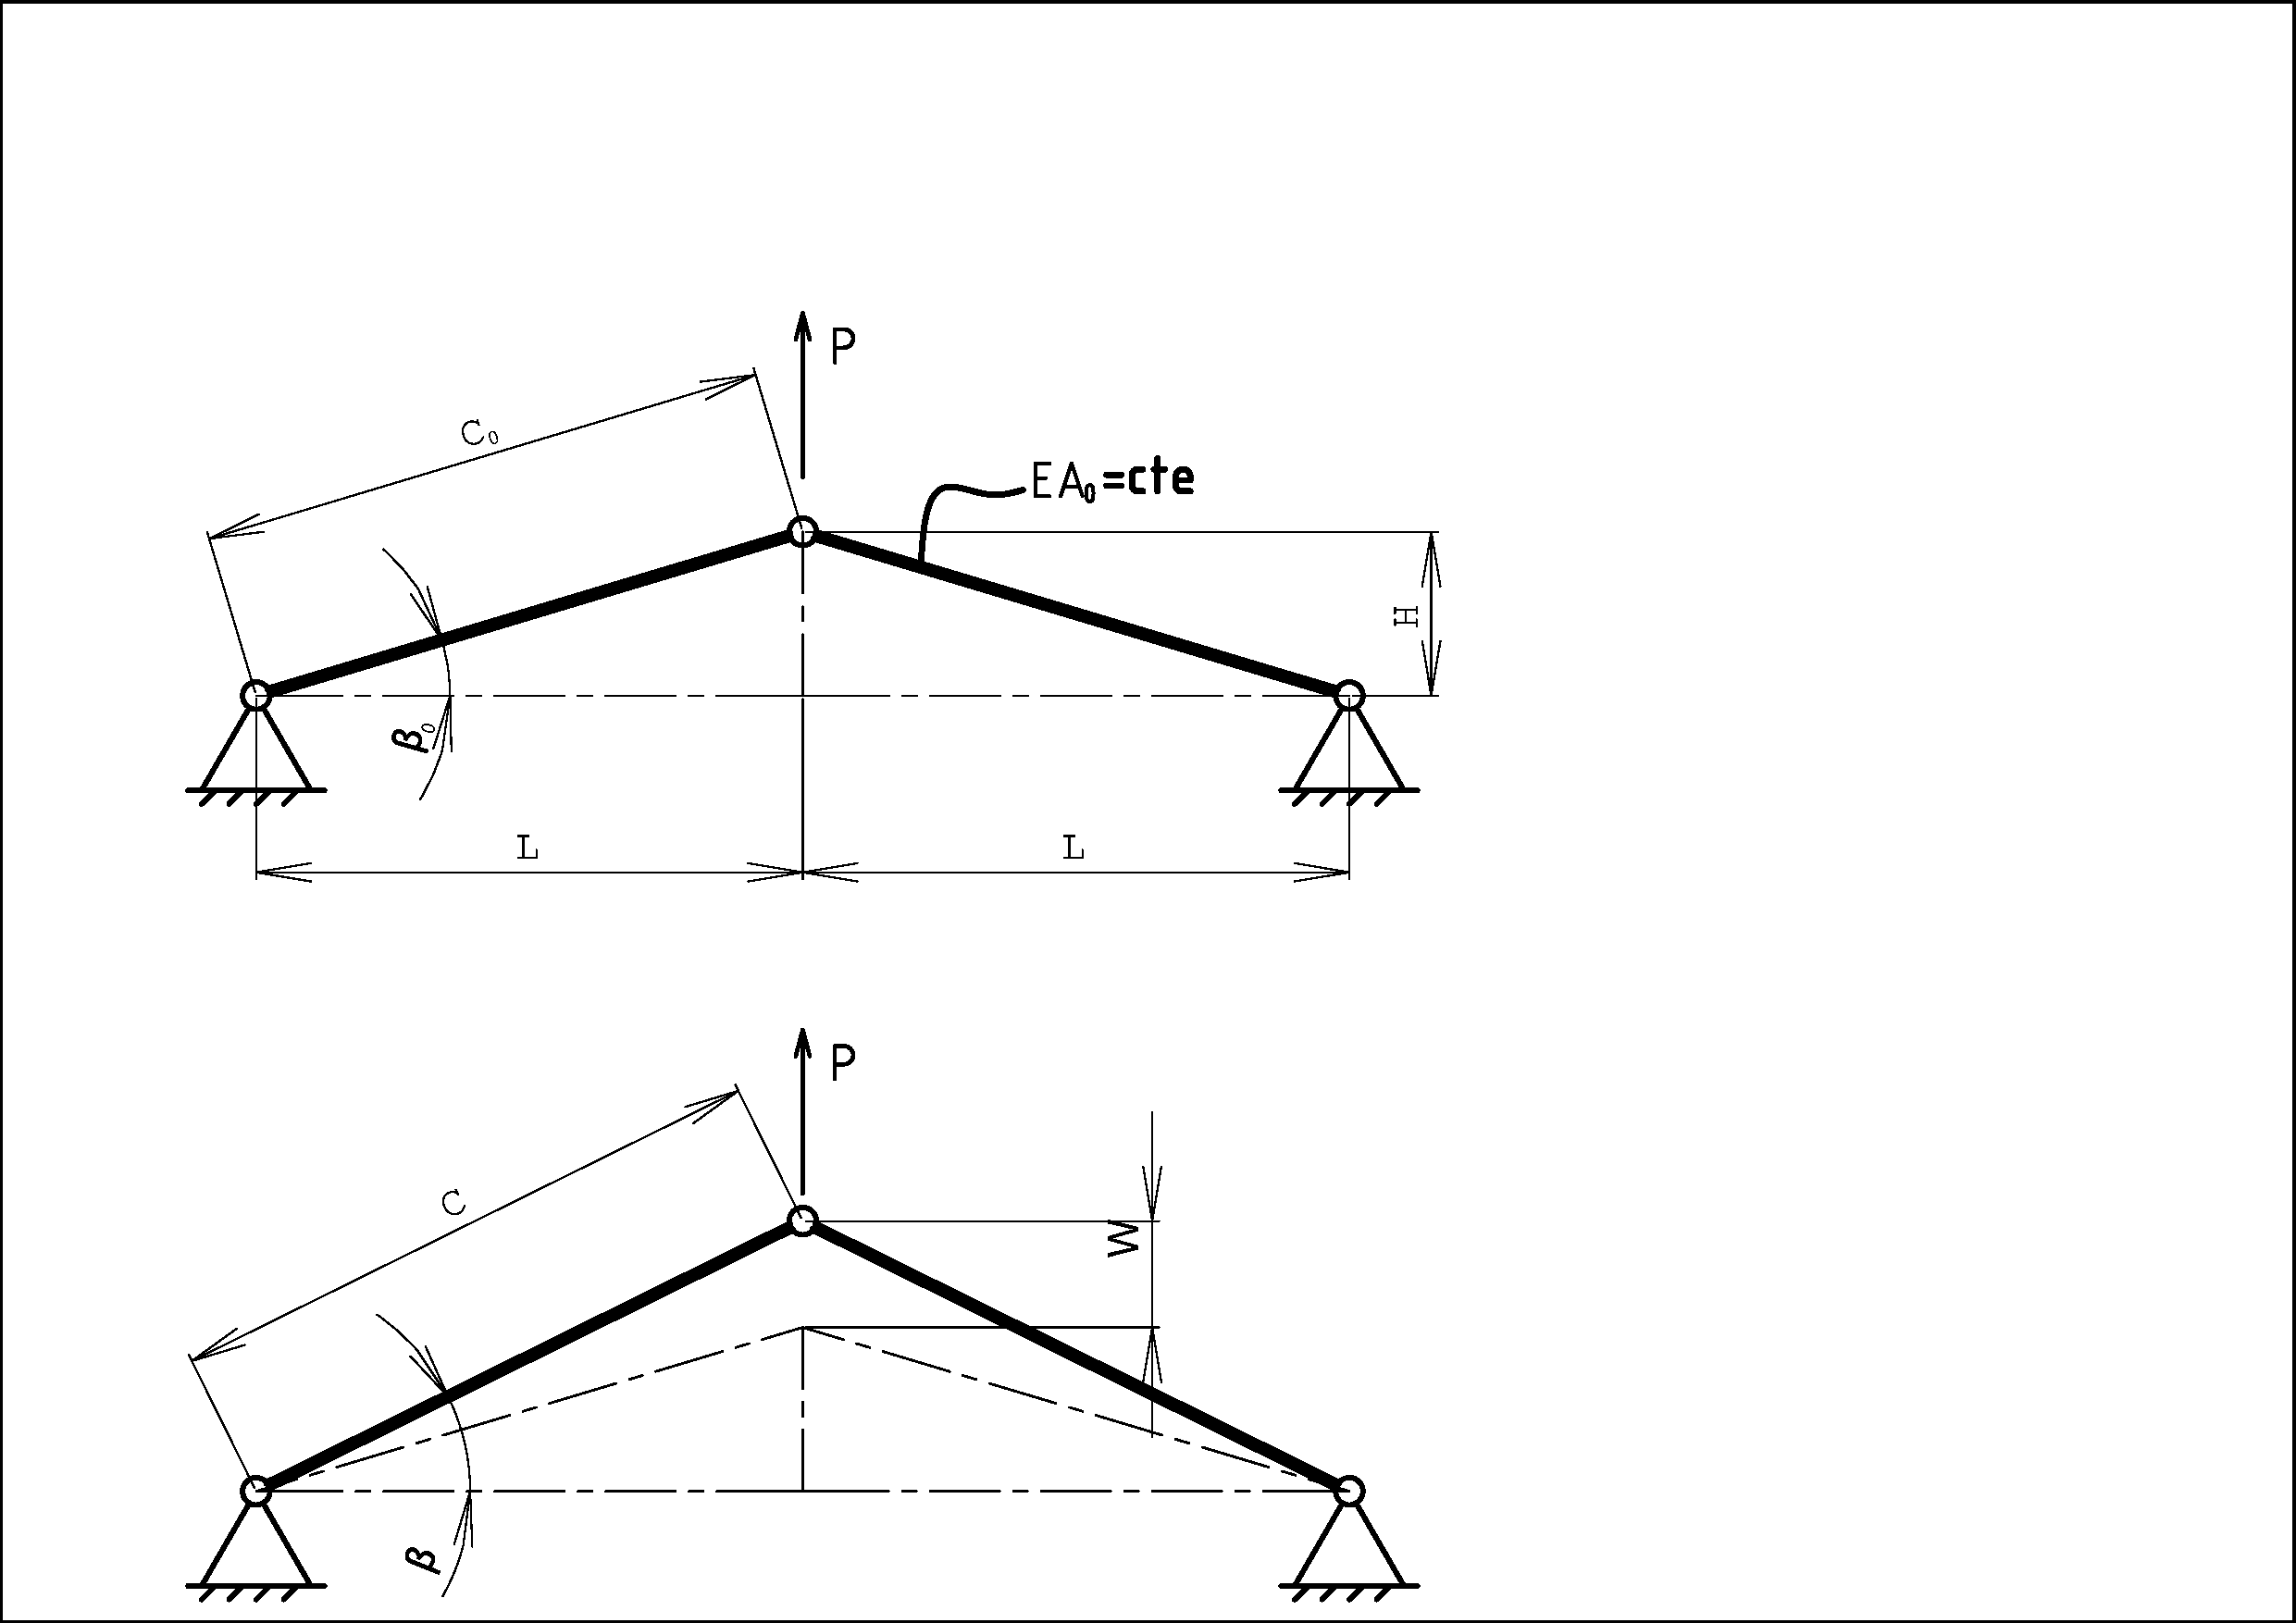
\includegraphics[
		trim=30mm 4mm 150mm 55mm,
		clip,
		width=0.6\textwidth
	]{figuras/TPs-9.pdf}
\end{figure}

$\longrightarrow$ Verificar a deformação final


% ================ Resolução TP-09 ================
\begin{textocaixa}
\hspace{10mm}





\end{textocaixa}
% ============================================== %

%%%%%%%%%%%%%%%%%%%%%%%%%%%%%%%%%%%%%%%%%%%%%%%%%%
%%%			  10 Trabalho Prático 10		   %%%
%%%%%%%%%%%%%%%%%%%%%%%%%%%%%%%%%%%%%%%%%%%%%%%%%%

% ============================================== %

\section{Trabalho Prático 10}

Ler e resumir o artigo:

\begin{center}
	YANG, Y. -B.; SHIEH, M. -S. (1990)

	\textit{"Solution method for nonlinear problems with multiple critical points."}

	AIAA Journal, V. 28, p. 2110-2116.
\end{center}


% ================ Resolução TP-10 ================
\begin{textocaixa}

\hspace{10mm}
O artigo de Yang e Shieh (1990) propõe um método aprimorado para a solução de problemas
não-lineares geométricos com múltiplos pontos críticos, denominado \textbf{Método de
Controle de Deslocamento Generalizado} (\textit{Generalized Displacement Control Method} --
GDC). O desenvolvimento se insere no contexto de análises estruturais nas quais a curva
carga-deslocamento exibe \textit{pontos limite} (onde a rigidez tangente se anula e o caminho
de equilíbrio muda de estável para instável) e \textit{pontos de retrocesso}
(\textit{snap-back points}), onde o próprio deslocamento de controle inverte de sentido.

\subsection*{Formulação no Espaço de Dimensão $N+1$}

A equação matricial que governa a $j$-ésima iteração do $i$-ésimo incremento de um sistema
com $N$ graus de liberdade é escrita como:

\begin{equation}
	[K]^{i}_{j-1}\{u\}^{i}_{j} = \lambda^{i}_{j}\{P\} + \{R\}^{i}_{j-1}
\end{equation}

Onde $[K]$ é a matriz de rigidez tangente, $\{u\}$ o vetor de incremento de deslocamentos,
$\{P\}$ o vetor de carga de referência, $\lambda$ o parâmetro de incremento de carga e
$\{R\}$ o vetor de forças desequilibradas. Como ambos $\{u\}$ e $\lambda$ são incógnitas,
uma equação de restrição adicional é necessária:

\begin{equation}
	\langle C \rangle \{u\}^{i}_{j} + k\,\lambda^{i}_{j} = H^{i}_{j}
	\label{eq:restricao_tp10}
\end{equation}

A seleção adequada das constantes $\langle C \rangle$, $k$ e $H^i_j$ na
\autoref{eq:restricao_tp10} é o ponto central que distingue os diferentes métodos de solução.
Os autores mostram que, para garantir estabilidade numérica, o parâmetro de incremento de
carga $\lambda^i_j$ deve permanecer limitado durante toda a análise. Por decomposição da
matriz de rigidez generalizada $[\bar{K}_1]$ no espaço $N+1$, obtém-se a expressão geral:

\begin{equation}
	\lambda^{i}_{j} = \frac{H^{i}_{j} - \lambda^{i}_{1}
					       \langle u_1 \rangle^{i-1}_{1}\{u_2\}^{i}_{j}}
						   {\lambda^{i}_{1}\langle u_1 \rangle^{i-1}_{1}\{u_1\}^{i}_{j}}
	\label{eq:lambda_tp10}
\end{equation}

Na qual $\{u_1\}^{i-1}_1$ é o vetor de deslocamentos resultante da primeira iteração do
último passo incremental.

\subsection*{Avaliação dos Métodos Existentes}

Os autores utilizam a Equação~\eqref{eq:lambda_tp10} como critério analítico para avaliar os
métodos clássicos:

\begin{itemize}
	\item \textbf{Newton-Raphson:} mantém $\lambda$ limitado nos passos iterativos, porém o
	incremento de deslocamento $\{u\}_j$ pode divergir próximo a pontos limite, pois
	$\det[K] \to 0$ nesses pontos.

	\item \textbf{Controle de Deslocamento:} contorna os pontos limite com sucesso, mas
	falha nos pontos de retrocesso: quando o deslocamento de controle $u^c$ tende a zero,
	$\lambda^i_j \to \infty$.

	\item \textbf{Comprimento de Arco (\textit{Arc-Length}):} pode gerar sinais incorretos
	para $\lambda$ nas proximidades de pontos de retrocesso com gradientes acentuados, além
	de não fornecer de forma automática a informação necessária para inverter a direção de
	carregamento.

	\item \textbf{Controle de Trabalho:} baseado no Parâmetro de Rigidez Atual (CSP --
	\textit{Current Stiffness Parameter}), que apresenta descontinuidades próximas a pontos
	de retrocesso e muda de sinal tanto em pontos limite quanto em pontos de retrocesso,
	sendo um indicador inadequado para a inversão de direção de carregamento.
\end{itemize}

\subsection*{Método Proposto: Controle de Deslocamento Generalizado}

Adotando $k = 0$ e $\langle C \rangle = \lambda^{i}_{1}\langle u_1 \rangle^{i-1}_{1}$ na
equação de restrição geral, obtém-se, para o passo incremental ($j=1$):

\begin{equation}
	\lambda^{i}_{1} = \lambda^{1}_{1}\left(\frac{\langle u_1 \rangle^{1}_{1}\{u_1\}^{1}_{1}}
								 {\langle u_1 \rangle^{i-1}_{1}\{u_1\}^{i}_{1}}\right)^{1/2}
	= \lambda^{1}_{1}\,(\text{GSP})^{1/2}
\end{equation}

E, para as iterações subsequentes ($j \geq 2$):

\begin{equation}
	\lambda^{i}_{j} = -\frac{\langle u_1 \rangle^{i-1}_{1}\{u_2\}^{i}_{j}}
							{\langle u_1 \rangle^{i-1}_{1}\{u_1\}^{i}_{j}}
\end{equation}

O \textbf{Parâmetro de Rigidez Generalizado} (GSP --
\textit{Generalized Stiffness Parameter}) é definido como:

\begin{equation}
	\text{GSP} = \frac{\langle u_1 \rangle^{1}_{1}\{u_1\}^{1}_{1}}
					  {\langle u_1 \rangle^{i-1}_{1}\{u_1\}^{i}_{1}}
\end{equation}

Onde o numerador representa os deslocamentos do primeiro passo e o denominador os do passo
atual. O GSP apresenta as seguintes propriedades fundamentais:

\begin{enumerate}
	\item Inicia com valor unitário e é nulo nos pontos limite, tal como o CSP;
	\item É negativo \underline{apenas} para os passos imediatamente após os pontos limite
	-- ao contrário do CSP, que muda de sinal também nos pontos de retrocesso --, tornando-o
	um indicador confiável e exclusivo para a inversão da direção de carregamento;
	\item Não apresenta descontinuidades numéricas nas proximidades de pontos de retrocesso,
	ao contrário do CSP, que exibe variações abruptas nessas regiões.
\end{enumerate}

\subsection*{Algoritmo}

O procedimento numérico do GDC pode ser sintetizado nas seguintes etapas:

\begin{enumerate}
	\item Definir o incremento de carga básico $\lambda^{1}_{1}$ para o início;
	\item Para a \textbf{primeira iteração} ($j = 1$) de cada passo $i$: montar
	$[K]^{i}_{0}$; resolver a equação de equilíbrio para $\{u_1\}^{i}_{1}$; calcular o GSP
	(para $i \geq 2$) e determinar $\lambda^{i}_{1}$; verificar o sinal do GSP -- se
	negativo, multiplicar $\lambda^{i}_{1}$ por $-1$ para inverter a direção de carregamento;
	\item Para \textbf{iterações subsequentes} ($j \geq 2$): calcular as forças
	desequilibradas; resolver os sistemas para $\{u_1\}^{i}_{j}$ e $\{u_2\}^{i}_{j}$;
	determinar $\lambda^{i}_{j}$ e atualizar $\{u\}^{i}_{j}$;
	\item Atualizar forças internas, nível de carregamento e geometria;
	\item Repetir até atingir a convergência e, se o carregamento total não exceder o
	máximo, avançar ao próximo incremento.
\end{enumerate}

\subsection*{Exemplos Numéricos}

Os autores validam o GDC em dois exemplos de referência:

\textbf{Exemplo 1 -- Treliça de von Mises}

\begin{figure}[H]
	\centering
	\caption{Treliça de dois membros.}
	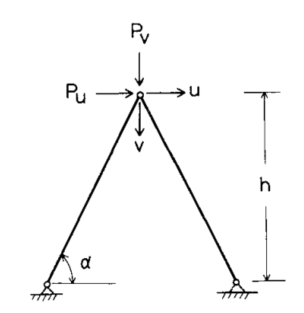
\includegraphics[
		width=0.3\textwidth
	]{figuras/TP10-ex1.png}
	\caption*{Fonte: Adaptado de YANG, Y. -B.; SHIEH, M. -S. (1990)}
	\label{fig:TP10-ex1}
\end{figure}

Para dois casos de carregamento (carga
horizontal como imperfeição: $P_u = 0{,}05\,P_v$; e carga vertical como imperfeição:
$P_v = 0{,}05\,P_u$), os resultados mostram curvas do tipo laço com quatro pontos limite
e dois pontos de retrocesso. O GDC rastreia o caminho completo de equilíbrio com sucesso,
invertendo automaticamente a direção de carregamento nos pontos limite. O GSP exibe
comportamento suave ao longo de toda a trajetória, enquanto o CSP apresenta descontinuidades
acentuadas nos pontos de retrocesso.

\begin{figure}[H]
	\centering
	\caption{Resultados gerais do Exemplo 1 para o primeiro caso de carregamento.}
	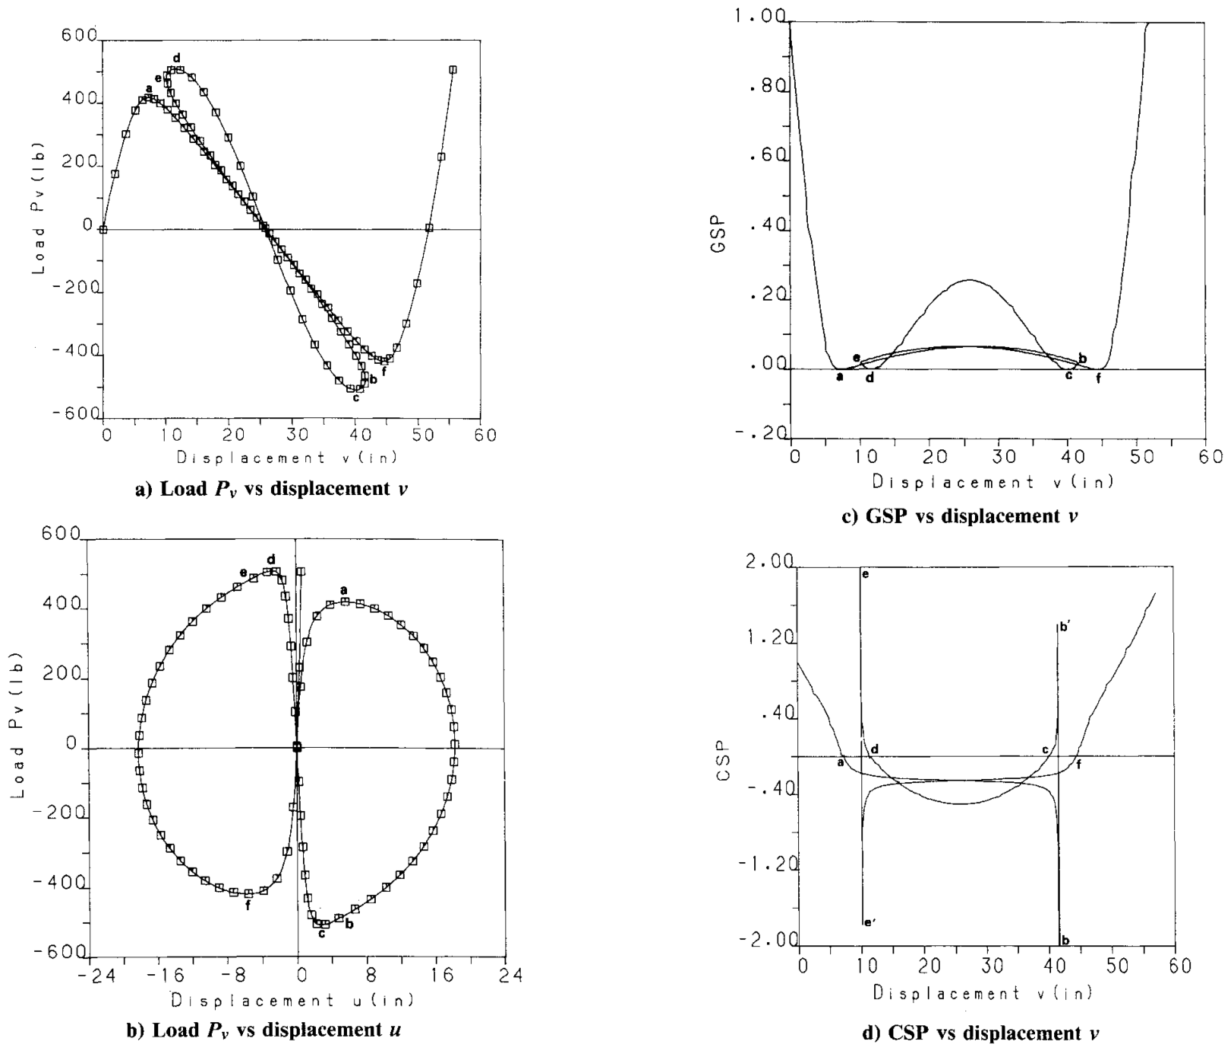
\includegraphics[
		width=\textwidth
	]{figuras/TP10-ex1_result1.png}
	\caption*{Fonte: Adaptado de YANG, Y. -B.; SHIEH, M. -S. (1990)}
	\label{fig:TP10-ex1_result1}
\end{figure}

\begin{figure}[H]
	\centering
	\caption{Resultados gerais do Exemplo 1 para o segundo caso de carregamento.}
	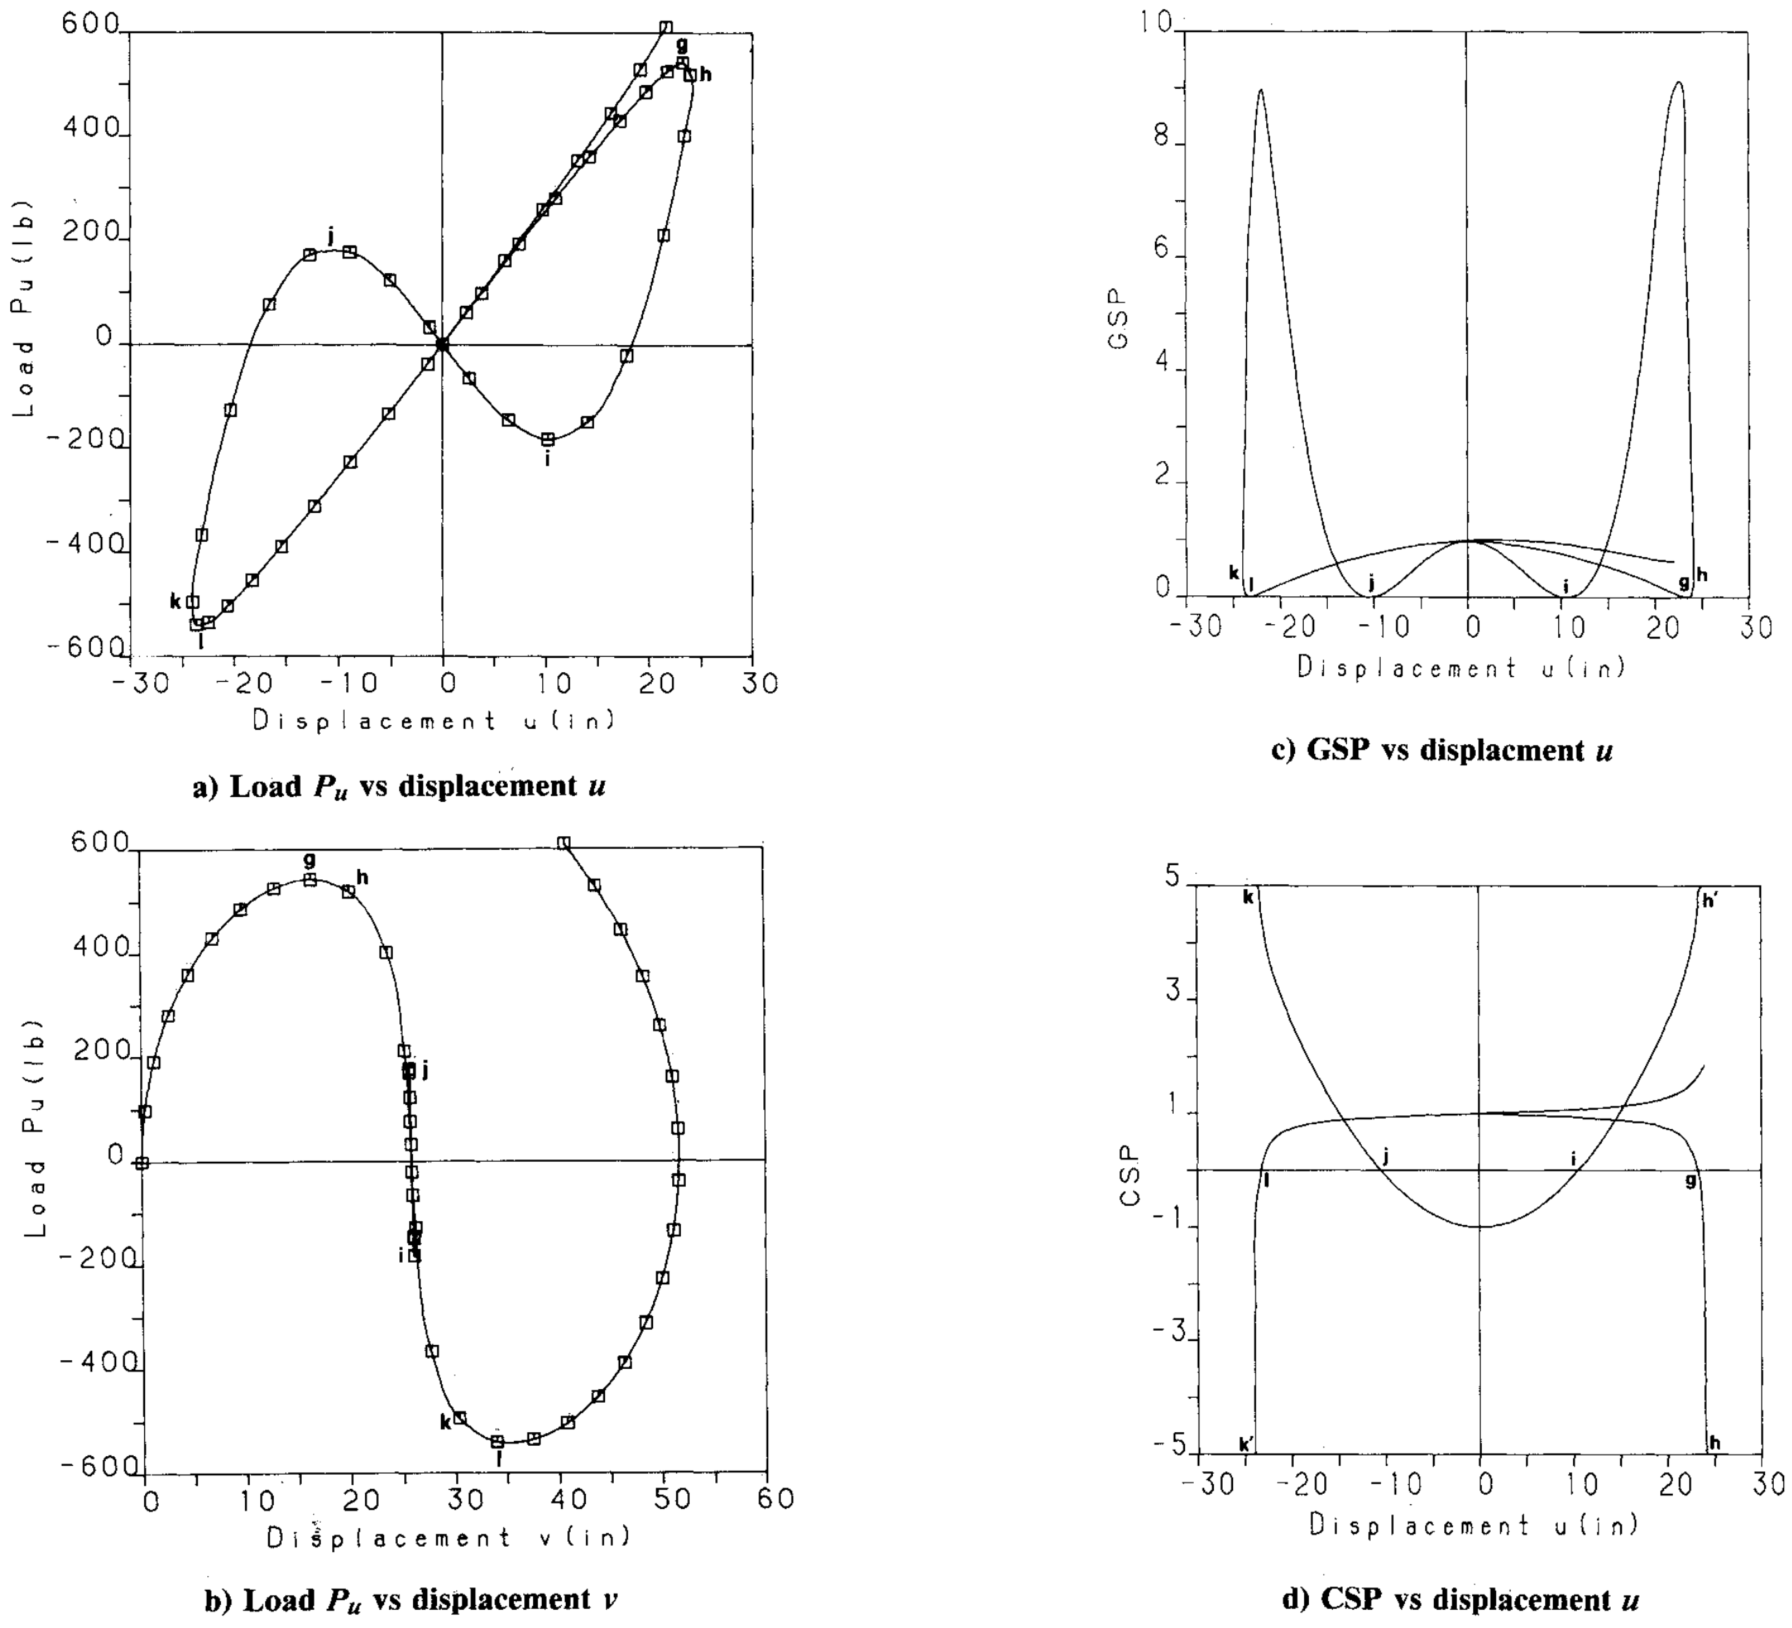
\includegraphics[
		width=0.95\textwidth
	]{figuras/TP10-ex1_result2.png}
	\caption*{Fonte: Adaptado de YANG, Y. -B.; SHIEH, M. -S. (1990)}
	\label{fig:TP10-ex1_result2}
\end{figure}

\textbf{Exemplo 2 -- Arco circular bi-articulado}

\begin{figure}[H]
	\centering
	\caption{Treliça de dois membros.}
	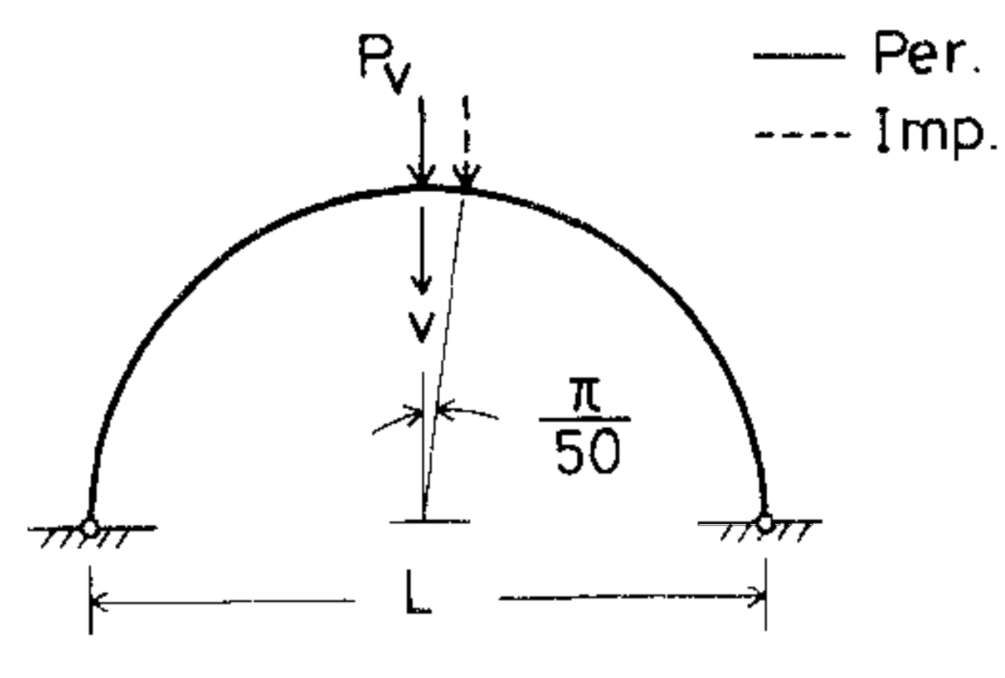
\includegraphics[
		width=0.4\textwidth
	]{figuras/TP10-ex2.png}
	\caption*{Fonte: Adaptado de YANG, Y. -B.; SHIEH, M. -S. (1990)}
	\label{fig:TP10-ex2}
\end{figure}

Representado por 26 elementos de viga
plana, o arco é submetido a carregamentos simétrico e assimétrico (com imperfeição de
posição). Os gráficos de carga-deslocamento exibem respostas de pós-flambagem com múltiplas
oscilações, demonstrando a capacidade do método de acompanhar trajetórias complexas com
grandes deformações.

\begin{figure}[H]
	\centering
	\caption{Resultados gerais do Exemplo 2.}
	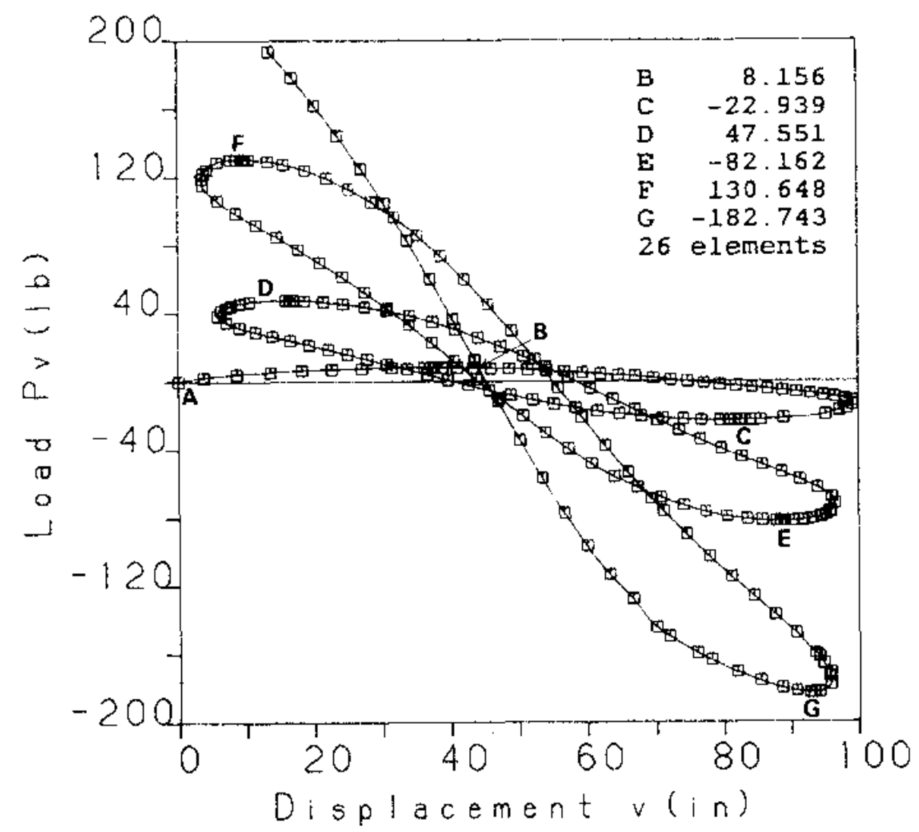
\includegraphics[
		width=0.6\textwidth
	]{figuras/TP10-ex2_result.png}
	\caption*{Fonte: Adaptado de YANG, Y. -B.; SHIEH, M. -S. (1990)}
	\label{fig:TP10-ex2_result}
\end{figure}

\subsection*{Conclusões}

O Método de Controle de Deslocamento Generalizado satisfaz simultaneamente os três
critérios fundamentais para métodos de solução não-linear:

\begin{enumerate}
	\item[(i)]   \textbf{estabilidade numérica} nas proximidades de pontos limite e de
	\textit{snap-back}, mantendo $\lambda^i_j$ e $\{u\}^i_j$ limitados;
	\item[(ii)]  \textbf{ajuste automático do tamanho dos passos} por meio do GSP, que
	reflete diretamente a variação de rigidez da estrutura ao longo da trajetória;
	\item[(iii)] \textbf{capacidade autoadaptativa} de inversão da direção de carregamento,
	usando o sinal do GSP como indicador exclusivo dos pontos limite. O método pode ser
	implementado diretamente em programas de elementos finitos de propósito geral para
	análise não-linear geométrica.
\end{enumerate}

\end{textocaixa}

%---------------------------------------------------------%
%                 ELEMENTOS PÓS-TEXTUAIS                  %
%---------------------------------------------------------%

%%%%%%%%%%%%%%%%%%%%%%%%% REFERENCIAS %%%%%%%%%%%%%%%%%%%%%%%%%%
% \newpage
% \phantomsection
% \addcontentsline{toc}{section}{\hspace{1.5cm}REFERÊNCIAS}
% \bibliographystyle{arquivos/custom.bst}
% \bibliography{pos-textuais/referencias.bib}

%%%%%%%%%%%%%%%%%%%%%%%%%% APÊNDICES %%%%%%%%%%%%%%%%%%%%%%%%%%%
% "Apêndices são conteúdos adicionais produzidos pelo autor"

% =================================== %

%%%%%%%%%%%%%%%%%%%%%%%%%%%%%%%%%%%%%%%
%%%         A APENDICE A            %%%
%%%%%%%%%%%%%%%%%%%%%%%%%%%%%%%%%%%%%%%

% =================================== %

\apendice{Rotinas numéricas implementadas para solução dos Trabalhos Práticos}
\label{apendice:A}




\subapendice{Trabalho prático 01}
\label{subapendice:TP01}





\subapendice{Trabalho prático 02}
\label{subapendice:TP02}





\subapendice{Trabalho prático 03}
\label{subapendice:TP03}





\subapendice{Trabalho prático 04}
\label{subapendice:TP04}





\subapendice{Trabalho prático 05}
\label{subapendice:TP05}





\subapendice{Trabalho prático 06}
\label{subapendice:TP06}





\subapendice{Trabalho prático 08}
\label{subapendice:TP08}





\subapendice{Trabalho prático 09}
\label{subapendice:TP09}

%%%%%%%%%%%%%%%%%%%%%%%%%%%%%%%%%%%%%%%%%%%%%%%%%%%%%%%%%%%
%                     FIM DO DOCUMENTO                    %
%%%%%%%%%%%%%%%%%%%%%%%%%%%%%%%%%%%%%%%%%%%%%%%%%%%%%%%%%%%
\end{document}